\documentclass[a4paper]{ltxdoc}

%% Fonts, etc.
%% Language and font encodings
\usepackage[english]{babel}

%% packages from beamer user guide
\usepackage{cmap}
\usepackage{lmodern}
\usepackage[T1]{fontenc}
\usepackage[utf8]{inputenc}
\usepackage{amsmath,amssymb}
\usepackage{pifont}
\usepackage{makeidx}
\usepackage{pgf,xcolor}
\usepackage[pdfborder={0 0 0},bookmarksnumbered]{hyperref}
\usepackage[left=2.25cm,right=2.25cm,top=2.5cm,bottom=2.5cm,nohead]{geometry}
\usepackage{translator}

\setcounter{tocdepth}{6}        %used for pgfbookmarks

%% more packages
\usepackage{tabularx}
\usepackage{etoolbox}
\usepackage{tikz}
\def\TikZ{Ti\textit{k}Z}

%% beamer userguide macros
\input{beamerug-macros}

\parskip0.5ex
\parindent0pt

\def\beamincr{\texttt{beamincr}}

\def\OR{\kern3pt\vrule width0.4pt height1.9ex depth0.9ex\kern3pt}%$\Big|$}
\def\meta#1{$\langle${\rmfamily\itshape#1}$\rangle$}
\def\ometa#1{\opt{\meta{#1}}}
\def\sarg#1{\texttt{<\meta{#1}>}}
\def\osarg#1{\opt{\sarg{#1}}}
\def\optsarg#1{\opt{\tt[\sarg{#1}]}}
\def\ott#1{\opt{\texttt{#1}}}
\def\offset{\opt{\meta{offset}}}
\def\ooffset{\opt{\texttt{(\meta{offset})}}}
\def\textpipe{\char`\|}

\makeatletter
\def\sanitisecommand#1{\expandafter\sanitisecommand@\string#1\nil}
\def\sanitisecommand@#1#2\nil{%
  \if#1\@backslashchar\expandafter\@firstoftwo\else\expandafter\@secondoftwo\fi%
     {\textbackslash#2}{#1#2}%
}
\makeatother
\def\ttx#1{\texttt{#1}}
\def\ttc#1{\texttt{\sanitisecommand#1}}
\def\cmd#1{\cmdlink{\stripcommand#1}{\texttt{\sanitisecommand#1}}}


%% indexing

% make a list of commands 
\makeatletter
\def\listofcommands{%
  \list{}{\leftmargin=2em\itemindent-\leftmargin\def\makelabel##1{\hss##1}}%
  \itemsep1ex%
  \@starttoc{loc}%
  \item{}%
  \endlist%
}
\def\addtoloc#1#2{%
  \@ifempty{#2}%
    {\addtocontents{loc}{\protect\item{\texttt{#1}\hfill\thepage}}}%
    {\addtocontents{loc}{\protect\item{\texttt{#1}\hfill\thepage}\\#2}}%
}
\def\locsection#1{\addtocontents{loc}{\vskip2ex\protect\item{\large \bf #1}}}
\makeatother


\makeatletter
% pop up a bookmark level -- this is copied from belowpdfbookmark
\def\poppdfbookmark{%
  \@tempcnta\Hy@currentbookmarklevel%
  \advance\@tempcnta by -1\relax%
  \xdef\Hy@currentbookmarklevel{\the\@tempcnta}%
}

% create a pdfbookmark, and write a macro to aux to remember the hypertarget (with level)
\def\pdfbkmktarget#1#2{%
  \belowpdfbookmark{#1}{#2}%
  \csxdef{@bookmark@#2}{#2.\the\numexpr\Hy@currentbookmarklevel+1\relax}%
  \protected@write\@auxout{}{\string\csgdef{@bookmark@#2}{#2.\the\numexpr\Hy@currentbookmarklevel+1\relax}}%
}
% link to the bookmark hypertarget
\def\cmdlink#1#2{%cmd target; text
  \hyperlink{\csuse{@bookmark@#1}}{#2}%
}
% add command to list of commands 
\def\addcmdtoloc#1#2#3{% bookmark target; cmd header; description
  \addtoloc{\string\hyperlink{#1.\the\numexpr\Hy@currentbookmarklevel+1\relax}{#2}}{#3}%
}
\makeatother

\def\bkmkcmd#1#2@#3{%
  \pdfbkmktarget{\sanitisecommand#1}{\stripcommand#1}%
  \addcmdtoloc{\stripcommand#1}{\sanitisecommand#1#2}{#3}%
}

\def\bkmkcmdalt#1#2#3#4{%
  \pdfbkmktarget{#1}{#2}%
  \ifblank{#4}{}{\addcmdtoloc{#2}{\sanitisecommand#3}{#4}}%
}

\def\bkmkenv#1#2{%
  \pdfbkmktarget{\textbackslash begin\{#1\}\dots\textbackslash end\{#1\}}{#1}%
  \addcmdtoloc{#1}{\textbackslash begin\{#1\}\dots\textbackslash end\{#1\}}{#2}%
}


% modify command environment to add toc entry
\let\oldcommand\command
\def\command#1#2{\bkmkcmd#1@{#2}\oldcommand{#1}}

% alt commands (don't usually start with \, and/or may need a simplified bookmark and/or hypertarget name)
\makeatletter
\newenvironment{commandalt}{\@ifnextchar[{\@commandalt}{\@commandalt@noopt}}{\endcommand}
\def\@commandalt[#1]{\@ifnextchar[{\@commandalt@twoopt[#1]}{\@commandalt@twoopt[#1][#1]}}
%\def\@commandalt@noopt#1{\pdfindxcmdalt{#1}{#1}\oldcommand{#1}}
\def\@commandalt@twoopt[#1][#2]#3#4{%
  \bkmkcmdalt{#1}{#2}{#3}{#4}%
  \oldcommand{#3}%
}
\makeatother

% continue the command name (formatting from beamerug-macros)
\def\contcmd#1{\declare{\texttt{#1}}}

% misspelt in beamerug-macros
\let\oldextractenvironment\extractenvironement
\def\extractenvironement#1#2@{\bkmkenv{#1}{}\oldextractenvironment{#1}#2@}

% adapt the environment doc macro to provide environment contents
\def\envwithcontents#1#2{%
  \list{}{\leftmargin=2em\itemindent-\leftmargin\def\makelabel##1{\hss##1}}%
  \extractenvwithcontents#1@{#2}\par\topsep=0pt}
\def\endenvwithcontents{\endlist}
\def\extractenvwithcontents#1#2@#3{%
  \bkmkenv{#1}{}%
  \item{{\ttfamily\char`\\begin\char`\{\declare{#1}\char`\}}#2}%
    {\itemsep=0pt\parskip=0pt%
      {\itemindent=-1em #3}%
    \item{\ttfamily\char`\\end\char`\{\declare{#1}\char`\}}%
    }%
  \index{#1@\protect\texttt{#1} environment}%
  \index{Environments!#1@\protect\texttt{#1}}}


%% Maths
\usepackage{amssymb,amsmath}

%% Citations, refs, hyperlinks
\usepackage[capitalize]{cleveref}


%% Title

\title{Enhanced \beamer\ increments:\\
the \texttt{beamincr} package}
\author{Maneesh Sahani}
\date{\today}


%% Document

\begin{document}

\maketitle

\noindent
The \beamincr\ package extends and enhances the incremental overlay mechanisms
implemented in the \beamer\ class.  These include labels to refer to and
manipulate overlay steps, an extended action syntax, and new increment-aware
environments.

\section{Background: overlays and increments}

The basic \beamer\ display unit is the \texttt{frame}.  A
frame may be rendered step-by-step, in which case the individual
versions of the frame are called ``overlays'' or ``slides''.  We will
use these terms interchangeably.
%
\beamer\ allows you to place material on an arbitrary slide in a frame like this
\example
\begin{verbatim}
\begin{frame}
  text on slides 1 and up\\
  \onslide<2->
  text on slides 2 and up\\
  \onslide<3-4>{
  text only on slides 3 and 4\\
  } 
  \only<5>{text only on slide 5\\}
  more text on slides 2 and up\\
\end{frame}
\end{verbatim}
You can read about the differences between \myprintcommand{onslide}
and \myprintcommand{only}, and the many other overlay-sensitive
commands, in the \beamer\ user guide.  Note in particular the
difference between the argument form and the declaration forms of
\myprintcommand{onslide}.  \myprintcommand{only} only works with an
argument.

This explicit numbering approach becomes burdensome when you want many overlays.
You have to keep track of the numbers explicitly, and if you subsequently add a
step early in the sequence you need to re-number the rest.  Thus, \beamer\ also
provides an incremental overlay specification.  The following code will produce
the same effect as that above.  \example
\begin{verbatim}
\begin{frame}
  \resetincr % not standard BEAMER
  text on slides 1+\\
  \onslide<+->
  text on slides 2+\\
  \onslide<+-+(1)>{ % increments counter by 1, despite the two +s
  text only on slides 3-4\\
  } 
  \onslide<+>{} % increment counter by another
  \only<+>{text only on slide 5\\}
  more text on slides 2+\\
\end{frame}
\end{verbatim}
This form allows easy automation using default overlay specifications.  For
instance (from the \beamer\ user guide) \example
\begin{verbatim}
\begin{itemize}[<+-| alert@+>]
\item Apple
\item Peach
\item Plum
\item Orange
\end{itemize}
\end{verbatim}
There are important and sometimes not-entirely-intuitive differences between the
incremental and explicit numbering systems.  So we will refer to the steps
implied in this way as ``increments''.  They will mostly match slide numbers,
but not always, as this example shows: \example
\begin{verbatim}
\begin{frame}
  \resetincr % not standard BEAMER
  text on slide 1+\\
  \onslide<3>{text on slide 3}\\
  text on slide 1+\\
  \onslide<+->
  text on slide 2+\\
  \onslide<4->
  text on slide 4+\\ % increment number is still 2!
  \onslide<+->
  text on slide 3+\\
\end{frame}
\end{verbatim}
The increments have their own internal logic (specifically, their own internal
counter) which is not affected by any explicit slide specifications that may
appear between incremental calls.  It may make sense to think of the increment
number as being associated with \emph{where} in the source file the material
appears, rather than (necessarily) on \emph{which slide} it appears.

There are a couple of oddities with the way increments work that often trip up
first-time users.  There are also some extensions that would be nice, like the
ability to refer to a specific increment elsewhere in the frame.  These things
are certainly possible in stock \beamer, but take some digging into internals.
The tools here make things a bit easier.

As an aside, \beamer\ has another incremental overlay system based on the
\cmd\pause\ command.  This uses the same counter as increments (in fact, the
counter is called \texttt{beamerpauses}), but inteprets it slightly differently. This
difference is discussed in \cref{sec:internals}. As a result, the two sets of
specifications don't play very well together, at least from the viewpoint of
non-experts.  More on this below.  I strongly suggest avoiding
\cmd\pause\ entirely when using \beamincr.


\section{Setting increments}\label{sec:setting}
\locsection{Increment labels and references}

\begin{command}{\resetincr\oarg{incrnum}}%
  {set increment to 1 or \meta{incrnum}}%
  %
  Reset the increment number to 1, or to the value defined by the optional
  argument if given.  This doesn't directly affect the slide on which any
  following text appears, but it does alter the effect of subsequent
  \texttt{<+>} or \texttt{<.>} increments (as well as the
  \cmdlink{/!/}{/!/} reference discussed below).  This command may be
  useful to synchronise overlays in (say) two columns or between highlighted
  bullet points and highlighting in a figure.  \example
\begin{verbatim}
\begin{frame}
  \resetincr
  \begin{center}
    Two lists \onslide<+->{in sync}
  \end{center}
  \begin{columns}
    \begin{column}{.2\textwidth}
      \begin{itemize}[<+-| alert@+>]
      \item Apple \item Peach \item Plum \item Orange
      \end{itemize}
    \end{column}
    \begin{column}{.2\textwidth}
      \resetincr[2] % restart the increment counter to sync
      \begin{itemize}[<+-| alert@+>]
      \item green \item yellow \item purple \item orange
      \end{itemize}
    \end{column}
  \end{columns}
\end{frame}
\end{verbatim}
Any optional argument must either be a number or be an increment reference
enclosed in \texttt{//} (these are defined in \cref{sec:labels}).  It cannot
specify any sort of range, or be \texttt+ or \texttt., although \texttt{/./} and
things like \texttt{/.(2)/} are allowed.

It is useful to call \cmd\resetincr\ at the start of every increment-based slide
(as we have in the examples here).  This avoids some potentially confusing
behaviour that comes from the way the increment counter is implemented in
\beamer:
\example
\begin{verbatim}
\begin{frame}
  text on slides 1-\\
  \onslide<+->
  text still on slides 1-\\
  \onslide<+->
  text on slides 2-
  \resetincr\onslide<.->
  text on slides 1-\\
  \onslide<+->
  text on slides 2-
\end{frame}
\end{verbatim}
The first call to \ttc{\onslide<+->} doesn't advance the slide, unless it
has been preceded by a \cmd\resetincr\ (or another \ttc{\onslide<+->} or a \cmd\pause).
\end{command}

\begin{command}{\fromincr\sarg{incrnum}}%
  {{\tt \textbackslash resetincr[\meta{incrnum}] \textbackslash onslide<.->}}%
  This is shorthand for
\begin{verbatim}
\resetincr[incr]
\onslide<.->
\end{verbatim}
It can only be used as a declaration (not with an argument).  The restrictions
on \meta{incr} are the same as above.  
\end{command}

\section{Labelling and referring to increments}\label{sec:labels}

In complicated frames, it may be useful to name certain increments for reference
elsewhere.  For instance, one might want to change a figure at certain steps
while progressing through a list of bullet points.  Or one might want to
redisplay certain slides in the frame with \cmd\againframe\ or
\cmd\handoutframe\ (described below).

\begin{command}{\incrlabel\osarg{incrnum}\marg{label}}%
  {attach \meta{label} to current increment or to \meta{incrnum}}%
\end{command}
\vskip-3ex
\begin{commandalt}[\textbackslash incrlabel=//][incrlabelslash]%
  {\incrlabel\osarg{incrnum}\opt{\meta{=}\dots}\texttt{/}\meta{label}\texttt{/}}%
  {attach \meta{label} to current increment or to \meta{incrnum}}%
%
  By default, this command attaches the current increment number to the label
  \meta{label}.  Once defined, the labelled increment can be recovered in
  (almost) any overlay spec using the constructs discussed below.  The
  \meta{label} can contain most characters, but should not start with \texttt{=}
  or contain any of \texttt{()-~}.  \hypertarget{label}{}%

  The \texttt= in the second form is optional, but if it is present then the
  \texttt{/\meta{label}/} may be separated from the \texttt= by additional
  material, which will be left in place.  The label must appear at the same
  grouping level as the \ttc{\incrlabel=} command and before the end of
  the current paragraph.  This is similar to the behaviour of the \texttt{=}
  action described in \cref{sec:actions:=}.

  If the optional \meta{incr} is provided, \meta{label} is set to its value.
  The restrictions on \meta{incr} are the same as for \cmd\resetincr: it
  can be a number or an increment specification.  This allows forms like
  \ttc{\incrlabel</.(2)/>{x}} to set \texttt x to the current increment +
  2.  See the discussion of increment specifications below.

  If \marg{label} starts with a number in parentheses (e.g. \texttt{(2)x}) then
  this number is added to the current increment, or to the value of \meta{incr},
  to obtain the label value.  Thus, the effect of the command above can also be
  achieved by \ttc{\incrlabel\{(2)x\}}.
\end{commandalt}

\begin{command}{\incrref \marg{incrref}}%
  {print increment value of \meta{incrref}}%
%
  This command returns the increment number defined by increment reference
  \meta{incrref} as described below.
\end{command}

\noindent
The general form of an increment reference is
\begin{commandalt}[<incrref>]{{ \meta{incrref}}: \meta{label}\ooffset}{}
%
  The label can be a string assigned by a call to \cmd\incrlabel, or be one of
  the following special characters:
  \begin{itemize}
  \item[\tt .]  \hypertarget{incrref.}{}The current increment (roughly
    equivalent to the incremental overlay specification `\ttx.', but can be used
    in places where only an \meta{incrref} is valid).

  \item[\tt \string^] \hypertarget{incrref^}{}The first overlay used in the
    frame.  This will usually evaluate to 1, but could be different if a slide
    range is specified for the frame.  It can be used to display text on the
    first slide shown, even if this is not slide 1.  For labelled frames (used
    with \cmd\againframe), the definition is tied to the label, and so will
    evaluate to the first overlay shown so far across all the uses of the frame.

  \item[\tt \string$] \hypertarget{incrref$}{}The last overlay (used) in the
    frame.  This is stored in the \ttx{.aux} file and so generally will only be
    correct after a second compilation.  It is tied to the frame label and so
    can be used to display only the final slide of a frame again:
    \cmd\againframe|</$/>{|\meta{frame label}|}|.  By combining with |^| it is
    possible to set a slide range at the first use and then automatically
    follow the same range with subsequent \cmd\againframe\ calls. \example
\begin{verbatim}
  \begin{frame}<2-5>[label=myframe] % only use slides 2-5 in this presentation
    ...
  \end{frame}
  ...
  \againframe</^/-/$/>{myframe} % show slides 2-5 again
  ...
  \againframe</$/>{myframe} % show only slide 5
\end{verbatim}

  \item[\tt \string$*] \hypertarget{incrref$*}{}The highest numbered overlay in
    the frame used so far.  This may be useful to have an
    \cmd\againframe\ command continue to display a partially rendered frame,
    starting from the latest overlay reached in any previous displays.

  \item[\tt \string@] \hypertarget{incrref@}{}The most recently displayed
    overlay number in the frame.  This may be useful to continue display
    picking up from where the last display left off.  
  
  \item[\tt !] \hypertarget{incrref!}{} The increment number set by the most
    recent \cmd\resetincr\ command (or reset action as introduced in
    \cref{sec:actions:!}).
  \end{itemize}
  The \meta{offset}, if given, is added to the increment indicated by the label.
  It can be negative.

  Increment references can be used as part of almost any overlay
  specification by enclosing them within slashes, e.g. \ttx{</foo(2)/>}.
\end{commandalt}
\example
\begin{verbatim}
\begin{frame}[label=twolists]
  \resetincr
  \begin{center}
    Two lists \onslide<+->{in sync}\\
    \onslide<+->{with more material\\}
    \onslide<+->{at the top}
  \end{center}
  \begin{columns}
    \begin{column}{.2\textwidth}
      \incrlabel{startlist}%
      \begin{itemize}[<+-| alert@+>]
      \item Apple \item Peach \incrlabel{halfway} \item Plum \item Orange
      \end{itemize}
    \end{column}
    \begin{column}{.2\textwidth}
      \resetincr[/startlist/]% keep in sync, even if we add extra topmatter
      \begin{itemize}[<+-| alert@+>]
      \item green \item yellow \item purple \item orange
      \end{itemize}
    \end{column}
  \end{columns}
  \vfill
  \onslide<+->
  The final increment is \incrref{.}. 
  \incrlabel{end}
\end{frame}
\end{verbatim}
%
\hypertarget{incrnum}{}%
Note that of commands discussed here, \cmd\incrref\ expects an \meta{incrref}
specification (i.e., \meta{label}\ooffset), while \cmd\resetincr,
\cmd\fromincr\ and \cmd\incrlabel\ expect an \meta{incrnum} specification that
might be an \meta{incrref} in \ttx{//} (i.e., \ttx{/\meta{label}\ooffset/}) or
just a number.  Standard overlay-aware commands should all accept overlay
specifications that include \meta{incrnum}s.

One \beamer\ command (slightly patched in this package) with which named
increments are particularly useful is \cmd\againframe.  So \example
\begin{verbatim}
  \againframe<1,/halfway/,/end(-1)/-/end/>{twolists}
\end{verbatim}
provides an abbreviated tour of the lists.  Increment labels are associated with
the label of the enclosing frame, and so the same names can safely be reused
across multiple named frames.

There is also a similar new command called \cmd\handoutframe\ to render more
than one overlay from a frame in \ttx{handout} or similar modes that otherwise
just show a single slide with all the overlays collapsed.  See \cref{sec:again}.

\section{Enhanced overlay action specifications}\label{sec:actions}

This section discusses further extensions to the overlay specification syntax,
and its interaction with increments and increment labels.
%
Many of these extensions are only valid in a context that supports
\beamer\ actions.  According to the user guide, these are \ttc\action,
\ttc\item, the \ttx{actionenv} environment and block environments like
\ttx{block} and \ttx{theorem}.  This package adds the fields of incremental
(\cref{sec:envs}) and incremental alignment (\cref{sec:align}) environments to
this list.  In the absence of any action specifications, \ttc\action\ acts like
\ttc\uncover.


\subsection{Setting increments in overlay action specifications} \label{sec:actions:!}

\begin{commandalt}[<resetincr@>]{{<resetincr@}\meta{incrnum}\contcmd{>}}{}
\end{commandalt}
\vskip-3ex
\begin{commandalt}[<!\meta{incrnum}>][<!incrnum>]{{<}\ott{\meta{incrnum}-}\contcmd!\meta{incrnum}\ott{-\meta{incrnum}}\contcmd{>}}{}
The current increment number can be reset using either the explicit
\ttx{resetincr@\meta{incrnum}} action, or an implicit \ttx{<!\meta{incrnum}>}
specification.  The \ttx!\meta{incrnum} may appear at either the start or end of
a (possibly open) range, so no more than one of the optional \ometa{incrnum}s
should be present.  To set to an intermediate value, use a specification like
\ttx{<1-4,!3>}.
%
\example
\begin{verbatim}
  \action<3-|resetincr@3>{body}
  \action<!3->{body}
\end{verbatim}
The increment number can be a label, with optional offset:
\begin{verbatim}
  \incrlabel<2>{x}
  \resetincr
  \action</x/->{body on 2+}
  \onslide<.->{this on 1+}
  \action<!/x(2)/->{body on 4+}
  \onslide<+->{this on 5+}
\end{verbatim}
The forms \ttx{<!+>} and \ttx{<!.>} aren't supported (and wouldn't be useful:
\ttx{<+>} already advances the increment, while \ttx{<!.>} would set it to its
current value).  However \ttx{<!/.(\meta{offset})/>} (note the \ttx/ label
notation) can be used to advance the increment counter by multiple (or negative)
steps.

The reset takes effect after the overlay specification has been interpreted and
before the body is set.  So any \ttx+ or \ttx. references will be relative to
the increment in effect \emph{before} the \ttc\action.
%
\pdfbkmktarget{}{/!/}%
%
However, the special increment label \ttx{/!/} can be used to access the most
recent reset (but note the discussion of evaluation order below).
%
\example
\begin{verbatim}
  \resetincr
  \action<!/.(2)/-|alert@.>{alerts too early}
  \action<!/.(2)/->{\alert<.>{alerts when uncovered}}
  \action<!/.(2)/-|alert@/!/>{alerts when uncovered}
\end{verbatim}

It is possible to issue multiple implicit and explicit resetincr action commands
in one overlay spec (including at both limits of a \meta{range}).  The increment
number in effect after the \meta{action spec} will be determined by the first
explicit \ttx{resetincr@} action, or if there are none, the first implicit
\ttx{!\meta{incrnum}} specification.

If any actions within the same \meta{action spec} depend on a \ttx{/!/}
increment reference, then this value will be determined by the \emph{following}
\ttx{resetincr@} value, or if there are none, the \emph{first}
\ttx!\meta{incrnum}, or if there are none, the most recent increment reset (by a
\cmd\resetincr\ command or an action).  If there are no preceding resets in the
frame, then \ttx{/!/} (along with any offset) evaluates to 0.  See the
discussion of \cmd\allowundefinedincrlabels\ for more on 0-valued references,
but note that this behaviour for \ttx{/!/} is independent of the
\cmd\allowundefinedincrlabels\ state.
%
\example
\begin{verbatim}
  \resetincr
  \action<1-5|resetincr@3|alert@/!/>{alerts on slide 1\\}
  \action<1-5|alert@/!/>{alerts on slide 3\\}
  \resetincr
  \action<1-5|alert@/!/|resetincr@3>{alerts on slide 3\\}
  \action<1-!5|point@/!/|resetincr@4|alert@/!/>{points on slide 4; alerts on slide 5\\}
\end{verbatim}

This ordering behaviour can be understood from the following two facts:
\beamer\ applies actions in the reverse order to that in which they appear in
the specification, and \beamincr\ maps \ttx{!\meta{incrnum}} specifications to
explicit actions at the \emph{end} of the \meta{action spec}, preserving their
order.

Actions must be used with argument text (usually enclosed in braces) or as
environments.  There is no equivalent to the declaration form of \ttc\onslide.
Note, however, that \cmd\fromincr\ (\cref{sec:setting}) implements an
\ttc\onslide\ declaration while also setting the current increment.  See also
the \cmdlink{incremental}{\tt incremental} environment
(\cref{sec:envs:incremental}).
\end{commandalt}

\subsection{Assigning labels from overlay action specifications} \label{sec:actions:=}

\begin{commandalt}[<=>/label/]{{<$\cdots$\textpipe=}\ooffset\contcmd{\textpipe$\cdots$>}%
    \ttx{\{\dots /\ooffset\meta{label}/ \dots\}}}{} This syntax can be used
  to assign a label using an action specification.  The name of the label to be
  assigned must be enclosed in \ttx{//}s within the \emph{argument} of the
  \ttc\action\ (or \ttc\item\ or \ttc\next\ or alignment field
  \dots)\footnote{\beamer\ actions don't make it possible to pass a text
  argument to the handler.}  The label is assigned to the increment number after
  any \ttx{+} or \ttx{!} actions have been interpreted, as though it was
  called with \cmd\incrlabel\ in place.  Thus in this code \example
\begin{verbatim}
  \resetincr[3]
  \action<!/.(2)/>{\incrlabel{x}action text}
  \resetincr[3]
  \action<!/.(2)/|=>{/x/action text}
  \resetincr[3]
  \action<!/.(3)/>{\incrlabel</.(-1)/>{x}action text}
  \resetincr[3]
  \action<!/.(3)/|=(-1)>{/x/action text}
  \resetincr[3]
  \action<!/.(3)/|=>{/(-1)x/action text}
\end{verbatim}
the first two action calls set the label \ttx{x} to 5.  The last three
illustrate the use of assignment offsets: if \ttx{=} is followed by a number
in parentheses, this is treated as an offset to add to the current increment at
assignment, in the same way as indicated by the optional
\ttx{<\meta{incrnum}>} argument to \cmd\incrlabel.  The same effect can
be achieved by placing the offset before the label name within the enclosing
\ttx{//}.

If no \ttx{/\meta{label}/} is found or if \meta{label} is empty, the action
tries to do nothing quietly.  This makes it possible to use an \ttx{=} in a
default spec, while only assigning a label on selected steps.  However, this
behaviour comes with warnings, and should be used with caution.  First, because
of the way \beamer's internals work, it is not currently possible to omit the
\ttx{//} in an \ttc\item, although the label can be empty (omission is fine in
the fields of an incremental or incremental alignment environment).  Second, if
there happens to be one more or more \ttx{/} characters in the argument to the
action, the text between them (or from a single \ttx{/} to the end) will be
interpreted as a label, unless they appear in a group within the argument, or an
explicit \ttx{//} pair appears first.  You have been warned!
\end{commandalt}


\subsection{Extending default overlay or action specifications} \label{sec:actions:~}
    
\begin{commandalt}[<\textasciitilde>][tilde]{}
Ordinarily, explicit overlay or action specifications override any defaults that
might apply.  It may sometimes be convenient to instead extend the default.  The
|~| spec can be used to add the current default spec fields into an explicit
overlay specification.  In this form, the \ttx\textasciitilde\ may be proceeded
by, say, a mode specification, but must not be followed by any text with the
specification field (i.e., to the next \ttx\textpipe\ or \ttx>).
%
\example
\begin{verbatim}
  \begin{itemize}[<+-| alert@+|=>]
  \item/ap/ Apple \item/pe/ Peach \item/pl/ Plum \item/or/ Orange
  \end{itemize}
  \begin{itemize}[<alert@/!/>]
  \item<!/pe/-|~> yellow \item<!/or/-|~> orange \item<!/ap/-|~>green \item<!/pl/-|~> purple
  \end{itemize}
\end{verbatim}
Within incremental alignment environments (\cref{sec:align}), a |~| will
incorporate the field-specific default.

This extension is available is any overlay specification.
\end{commandalt}

\begin{commandalt}[<defaultspec@>]{{<defaultspec@}\meta{range}\contcmd{>}}{}

  Action to set the default specification for overlay references within the
  action argument.  The \meta{range} may be any valid specification for a set of
  slides (such as \ttx{1}, \ttx{+-} or \ttx{!/foo/-/bar/}).  The range is
  evaluated within the context of the \ttx{defaultspec@} specification, yielding
  specific slide numbers.  Thus, any labels (including \ttx{/./} and \ttx{/!/})
  or \ttx+ or \ttx. symbols will be replaced by their current values.  For
  example, in
\begin{verbatim}
  \resetincr[3]
  \action<+-|defaultspec@+>{\only<~>{only body} other stuff}
\end{verbatim}
  the specification to \ttc\only\ is set to \ttx{<4>}, not to
  \ttx{<+>}, which would evaluate to slide 5 in context.  See also the
  \ttx\textasciitilde\ action below.
\end{commandalt}

\begin{commandalt}[<\textasciitilde range>][tilde range]{{<\textasciitilde}\meta{range}\contcmd{\textpipe$\cdots$>}}{}

  This is equivalent to \ttx{<\meta{range}\textpipe
    defaultspec@\meta{range}\textpipe$\cdots$>}.  That is, it executes the
  calling action on \meta{range} (using normal overlay evaluation rules) and
  also sets the default specification within the action argument to the
  evaluated range.
  %
  This extension only works in an action specification context.  As the body of
  the argument will usually only be visible for the specified range anyway, the
  specification is most useful to control side effects.
  \example
\begin{verbatim}
  \resetincr
  \setcounter{displayed}{0}
  \begin{itemize}[<+->]
  \item \only<~>{\stepcounter{displayed}} % \only<+-> adds another increment
  \item<~+-> \only<~>{\stepcounter{displayed}} % \only<4-> does not
  \item<~~> \only<~>{\stepcounter{displayed}} % \only<5-> does not
  \end{itemize}
\end{verbatim}
    In the example, the \ttc\only\ commands are used to advance the counter on
    slides where the \ttc\item s are visible.  In both cases the overlay
    specification to \ttc\only\ is a copy of the surrounding default
    specification.  For the first one, this is \ttx{<+->}.  For the second, it
    is \ttx{<+->} \emph{evaluated} within the \ttc\item\ call, giving
    \ttx{<3->}.  The final case expands the second |~| to the default \ttx{+-},
    which becomes the increment specification for the item, and then sets the
    default within the item to its value, which is \ttx{5-}.
\end{commandalt}


\subsection{Advanced references: using labels defined later} \label{sec:actions:advanced}

\begin{command}{\allowundefinedincrlabels\oarg{flag}}%
  {control whether undefined labels generate errors or  evaluate to 0}
  %
  If called alone, or with option \meta{\opt{flag}} > 0, tells \LaTeX\ not to
  generate an error when encountering an undefined increment label.  References
  to such labels instead evaluate to 0, and any offset in the reference is
  ignored.  If \meta{\opt{flag}}=0, the default error-generating behaviour is
  restored.
\end{command}
If a referenced label is defined later in the same frame, then it will take on
that later-defined value on subsequent slides of the frame.  Thus, in effect,
this option makes it possible to refer to increment labels before they are
defined.  (Although material intended to be set on slide 1 cannot depend on such
advance references.)

If the label is used as part of an open range then it may be necessary to use a
special syntax in which the range indicator is placed \emph{within} the
\ttx{/ /} enclosing the label.  If the label is undefined (and so 0), this
syntax sets the other limit of the range to 0 as well.  \example
\begin{verbatim}
  % /foo/ is not defined on first evaluation
  \onslide</foo/->{spec expands to <0->, so text appears on all slides}
  \onslide</foo-/>{spec expands to <0-0>, so text is suppressed}
  \incrlabel<2>{foo} % on later evaluations, both specs will expand to <2->
\end{verbatim}
If the range is closed with an explicit numerical or (defined) label upper
limit, then there is no current way to suppress early expansion.  However forms
like \ttx{/foo/-/foo(2)/} will evaluate to \ttx{0-0} as offsets are
ignored for undefined labels.

Many problems with advanced references (including range expansion and the
rendering of first-slide material) can be resolved by use of
\cmd\framescanonly\ and \cmd\againframe\ (\cref{sec:again}).

An \cmd\allowundefinedincrlabels\ command also makes it possible to
\emph{set} the current increment to an (initially) undefined label value using
\cmd\resetincr, \cmd\fromincr, or \ttx{<!/label/>}, thereby
setting the current increment to 0.  Text set on that increment will not appear
until the label is defined.  However, any subsequent \ttx{<+>} specs will
still advance the increment number, which may not be desired.  This behaviour
can be avoided by using the form \ttx{<!/.(1)/>} instead of \ttx{<+>}.
The current increment label \ttx{/./} is treated in the same way as an
undefined one when the increment is 0, and so the offset is ignored.  \example
\begin{verbatim}
\resetincr{/foo/} % no list items appear until /foo/ is defined
\begin{itemize}<!/.(1)-/|alert@/!/>
\item foo
\item bar
...
\end{itemize}
\end{verbatim}
If an initially undefined label is used to set the increment counter early in
the frame, then increment labels that are defined later in the frame may change
value once that first label is defined.  This can be used for powerful effects,
in which overlays in two different sections of the frame each depend on
increments from the other.  However, if the definition label used in the early
reference is itself altered by the change in that early evaluation, then there
is a risk of creating an infinite loop.
\example
\begin{verbatim}
  \begin{itemize}[<alert@/!/>]
  \item<!/./-     |~|=(1)>/ping/ Apple  % 1- (!/./ ensures alert occurs on same slide)
  \item<!/pong-/  |~> Peach             % 4-
  \item<!/.(1)-/  |~|=>/ping2/ Plum     % 5-
  \item<!/pong2-/ |~> Orange            % 8-
  \end{itemize}
  
  \begin{itemize}[<alert@/!/>]
  \item<!/ping-/  |~> green             % 2-
  \item<!/.(1)-/  |~|=(1)>/pong/ yellow % 3-
  \item<!/ping2-/ |~> purple            % 6-
  \item<!/.(1)-/  |~|=(1)>/pong2/orange % 7-
  \end{itemize}
\end{verbatim}



\section{Incremental environments}\label{sec:envs}

The \beamincr\ package provides some new increment-aware environments.  These
are described in the present section.  It also makes it possible to use
increment specifications within alignment environments such as \ttx{tabular} or
\AmSTeX\ \ttx{align}; these are discussed in \cref{sec:align}.

Each new environment is accessible under two, otherwise equivalent, names.  A
common base name is either preceded by the word \ttx{incremental} or followed
by the symbols \ttx{<>}.  The environments in this section separate material
into overlays using the token \ttc\next\ or \ttc{\next*}.  Many will
also apply an implicit or explicitly defined command to that material when
\ttc\next\ is used, but omit the command for \ttc{\next*}.

Each environment makes it possible to specify a default overlay specification,
applied to all \ttc\next\ fields, unless overridden by a local value.  If no
default is specified it is taken to be \ttx{<+->} (rather than any enclosing
default), since it is assumed that \ttx{incremental} environments are intended
to be, well, incremental.

Also in each case, a counter called \ttx{next} is set to 0 in the pre-next field
and then advanced at every \ttc\next.  An increment label called
\ttx{next\,\meta{n}}, where \meta{n} is the value of the \ttx{next} counter, is
defined immediately after each \ttc\next, before any contents are processed.
The label contains a (single) space before the number.


\subsection{Standard incremental environments}\label{sec:envs:incremental}
\locsection{Incremental environments}
\tracingmacros1
\begin{envwithcontents}{{incremental}\optsarg{default specification}}
  {\item \hskip1em \osarg{pre-next specification} \opt{\meta{pre-next contents}}
    \item \ttx{\string\next}\osarg{next specification}
    \item \hskip1em \meta{next contents}
    \item \ttx{\string\next}\osarg{next specification}
    \item \hskip1em \meta{next contents}
    \item \hskip2em $\vdots$
  }
  This environment can be thought of as an increment-aware \ttx{itemize}
  without the list formatting.  This makes it suitable for incremental control
  of a wider range of types of code, such as \TikZ\ drawing commands.
%
  The keyword \ttc\next\ within the environment acts like
  \ttc\item\ in terms of incremental processing: the \meta{next contents}
  are set within an \ttc\action\ command.  Each \ttc\next\ call can
  be followed by an optional \osarg{next specification}, which is applied to the
  \meta{next contents}.  If the specification is omitted, then the environment
  \ometa{default specification} is applied.  If no \meta{default
    specification} was given in the environment, then the default is assumed to
  be \ttx{<+->}.

  Unlike in \ttx{itemize} environments, code can also appear before the first
  \ttc\next.  If any does, it is processed with the action specification given
  by \osarg{pre-next specification} if present, or else a default specification
  of \ttx{<.->} (to use the default specification defined for the environment,
  set \osarg{pre-next specification} to |<~>|).  On the other hand, if nothing
  but whitespace appears between the opening of the environment---or the
  optional default overlay spec---and the first \ttc\next, then no action is
  applied.  
  \example
\begin{verbatim}
\resetincr
\begin{incremental}[<+->]
  <.-> this text on slide \incrref{next 0} (=1);
\next
  on slide \incrref{next 1} (=2);
\next<!/.(2)/->
  on slide \incrref{next 2} (=4), after \thenext\ (=2) next commands.
\end{incremental}
\end{verbatim}
\end{envwithcontents}
\begin{environment}{{<>}\optsarg{default specification}}
  This is a synonym for |\begin{incremental} ... \end{incremental}|.
\end{environment}
%
The following environments apply a specified command to each overlay contents.

\begin{envwithcontents}{{incrementaldo}\marg{code}\optsarg{default specification}}
  {\item \hskip1em \osarg{pre-next specification} \opt{\meta{pre-next contents}}
    \item \ttx{\string\next}\osarg{next specification}
    \item \hskip1em \meta{next contents}
    \item \ttx{\string\next}\osarg{next specification}
    \item \hskip1em \meta{next contents}
    \item \hskip2em $\vdots$
  }

  This environment applies the command(s) in \meta{code} to each \meta{next
    contents}.

  If \meta{code} does not contain any |#| characters, \meta{next contents} is
  placed within a single group following it (as in \meta{code}\marg{next
    contents}).  Thus, if \meta{code} ends in a command that accepts one
  argument, that command will be applied to the contents.

  If \meta{code} does contain any |#|s then it is assumed to be the definition
  of a command taking a single argument that should be replaced by \meta{next
    contents} in the usual way.  As the command definition happens deep within
  the bowels of \beamer\ processing, the argument generally needs to be accessed
  as |####1|, \emph{unless} the enclosing frame is declared to be \ttx{fragile}
  (in the frame options), in which case just |#1| is needed.  This behaviour is
  triggered by \emph{any} |#| characters in \meta{code}, even if they are used
  in a non-argument context (the input is detokenised before being scanned for
  |#|s).  Thus if there is an ``incidental'' |#| without any reference to |#1|,
  then \meta{next contents} will be suppressed.

  The \meta{code} is skipped for any fields preceded by \ttc{\next*} in place of
  \ttc\next.  Contents following \ttc{\next*} is set in the same way as in a
  plain \ttx{incremental} environment.

  Any non-empty \meta{pre-next contents} is always processed without \meta{code}.
  
\end{envwithcontents}
\begin{environment}{{do<>}\marg{code}\optsarg{default specification}}
  This is a synonym for |\begin{incrementaldo} ... \end{incrementaldo}|.
\end{environment}


\begin{envwithcontents}{{incrementaldocmd}
    \oarg{num args}\marg{code}\optsarg{default specification}}
  {\item \hskip1em \osarg{pre-next specification} \opt{\meta{pre-next contents}}
    \item \ttx{\string\next}\osarg{next specification}
    \item \hskip1em \meta{next contents}
    \item \ttx{\string\next}\osarg{next specification}
    \item \hskip1em \meta{next contents}
    \item \hskip2em $\vdots$
  }

   This version inserts \meta{code} after each \ttc\next\ and before \meta{next
     contents} without grouping.  Thus, if \meta{code} is (or ends with) a
   command that takes one or more arguments, these will be read from the
   beginning of \meta{next contents}.  Braces may be needed within the contents
   to delineate the arguments.

   If the optional \opt{\meta{num args}} is non-zero, then this number of
   arguments is read from the text following \ttc\next\ and can be accessed
   using argument parameters (almost) as in \ttc\newcommand.  As the command
   evaluation happens deep within the bowels of \beamer\ processing, the
   parameter numbers must be protected with four |####| symbols, \emph{unless}
   the frame is declared to be \ttx{fragile} (in the frame options) in which
   case a single |#| is needed.

  Execution of \meta{code} can be avoided for specific fields by using
  \ttc{\next*} in place of \ttc\next.  Contents following \ttc{\next*} are set
  in the same way as in a plain \ttx{incremental} environment.

  Any non-empty \meta{pre-next contents} is always processed without
  \meta{code}.

  \example
\begin{verbatim}
\tikz[every node/.style={above,allow upside down,sloped}]{
  \begin{incrementaldocmd}[1]{\draw ({72*\thenext-72}:10ex)--(72*\thenext:10ex) node[midway] (####1) {####1};}
    [<+-|alert@+|=>]
    \next/one/   {one}
    \next/two/   {two}
    \next/three/ {three} \node[left] at (three.south) {\thenext/\theincrement};
    \next/four/  {four}
    \next/five/  {five}
    \next*/done/ \draw (0:5ex) \foreach \t in {1,...,5}{ -- (\t*72:5ex)};
                 \node [anchor=center] {done!};
  \end{incrementaldocmd}}
\end{verbatim}
\end{envwithcontents}
\begin{environment}{{docmd<>}
    \oarg{num args}\marg{code}\optsarg{default specification}}
  This is a synonym for |\begin{incrementaldocmd} ... \end{incrementaldocmd}|.
\end{environment}


\begin{envwithcontents}{{incrementaldodef}
    \oarg{parameter spec}\marg{code}\optsarg{default specification}}
  {\item \hskip1em \osarg{pre-next specification} \opt{\meta{pre-next contents}}
    \item \ttx{\string\next}\osarg{next specification}
    \item \hskip1em \meta{next contents}
    \item \ttx{\string\next}\osarg{next specification}
    \item \hskip1em \meta{next contents}
    \item \hskip2em $\vdots$
  }
  This is similar to the \ttx{incrementaldocmd} environment, but allows 
  arguments to be specified using the flexible format of \ttc\def.  Parameter
  numbers must be escaped with four |#|s in both specification and code, unless
  the frame is declared \ttx{fragile}.  Code execution can be skipped using \ttc{\next*}
  and is always skipped for any \meta{pre-next contents}.
\end{envwithcontents}
\begin{environment}{{dodef<>}
    \oarg{parameter spec}\marg{code}\optsarg{default specification}}
  This is a synonym for |\begin{incrementaldodef} ... \end{incrementaldodef}|.
\end{environment}

\begin{environment}{{incrementaldolongdef}
    \oarg{parameter spec}\marg{code}\optsarg{default specification}}

  This form allows paragraph breaks within \meta{next contents}, but is
  otherwise the same as \ttc{\begin\{incrementaldodef\}} \ttx{...}
  \ttc{\end\{incrementaldodef\}},
\end{environment}
\begin{environment}{{dolongdef<>}
    \oarg{parameter spec}\marg{code}\optsarg{default specification}}
  This is a synonym for |\begin{incrementaldolongdef} ... \end{incrementaldolongdef}|.
\end{environment}


\subsection{\TikZ-based incremental environments}\label{sec:envs:tikz}

The following environments use \TikZ\ picture commands to create their effects.
They will only be defined if \TikZ\ is also loaded in the document preamble.

\begin{envwithcontents}{{incrementallayers}
    \oarg{node options}\optsarg{default specification}}
  {\item \hskip1em \osarg{pre-next specification} \opt{\meta{pre-next \TikZ\ commands}}
    \item \ttx{\string\next}\osarg{next specification}\oarg{next node options}
    \item \hskip1em \meta{layer contents}
    \item \ttx{\string\next*}\osarg{next specification}\oarg{scope options}
    \item \hskip1em \meta{\TikZ\ commands}
    \item \hskip2em $\vdots$
  }

  Set \meta{next contents} within overlayed \TikZ\ nodes.  This may have the
  effect of later text appearing to be layered on top of earlier material.  If
  the specifications place material on mutually exclusive increments (e.g. with
  \ttx{<+>}) then this has a similar effect to \beamer's \ttx{overprint}
  environment.  In particular, the region occupied by the environment will
  correspond to the largest of the nodes.  However, this behaviour can be
  subverted by use of \ttc\only\ or similar commands within the \meta{next
    contents}, or \ttx{only@} actions in \meta{next specification}s; these
  should be used with care.

  By default, nodes are set with \ttx{text width=\ttc\columnwidth, inner
    sep=0pt} so that the text fills the width of the current frame or column or
  minipage.  They are aligned at their top borders.  These defaults can be
  overridden, and arbitrary \TikZ\ options provided to the nodes, in one of
  three ways: by setting options in the \ttx{incremental layer} \TikZ\ style, by
  placing them in the optional \meta{node options} argument to the environment,
  or by placing them in the optional \meta{next node options} after a \ttc\next
  (and after any \meta{next specification}).

  Three shorthand node alignment keys are available: \ttx t aligns the nodes at
  their top edges (the default); \ttx{b} at their bottom edges and \ttx{c} at their
  centres.

  The entire environment is set within a single \ttx{tikzpicture}.  Any
  \meta{pre-next contents} and the contents of any \ttc{\next*} are interpreted
  as \TikZ\ commands within that picture.  Each \ttc{\next*} sets its contents
  within a \TikZ\ \ttx{scope} environment.  Options to this environment can be
  provided by starting the contents (after any \ometa{next specification}) with
  \oarg{scope options}.

  The default origin of the \TikZ\ coordinate system is the \ttx{north},
  \ttx{center} or \ttx{south} anchor points of the layer nodes for \ttx t, \ttx
  c and \ttx b alignment respectively.  The nodes themselves are accessible
  under the names \ttx{(layer \meta{n})}, where \meta{n} is the corresponding
  value of the |next| counter.

  \subpdfbookmark{layer scope options}{layer scope}
  The following special options can be given within \ttc{\next*} scope options.
  \begin{commandalt}[t c b (layer scope option)]{{t\OR c\OR b}}{}
      These options do not alter anything by themselves.
      However, subsequent calls to the options below will behave differently for
      different alignment keys.  The default value is the alignment of the most
      recent layer node.
  \end{commandalt}

  \begin{commandalt}[layer xy (layer scope option)]{{layer xy}\opt{=\meta{bbox}}}{}

    Set the \ttx{xy} coordinate system in the scope to span the bounding box of
    the layers rendered so far, or a specified \ometa{bbox} node.  It is
    possible to set \ometa{bbox} to \ttx{current page}, in combination with an
    \ttx{overlay} option to the scope.
%
    The origin of he coordinates depends on the alignment of the most recent
    layer, or a \ttx{t\OR c\OR b} alignment option to the \ttc{\next*} scope.
    The origin is placed at the \ttx{north west}, \ttx{center} or \ttx{south
      west} of the bounding node, for \ttx t, \ttx c, or \ttx b alignment
    respectively.  The \ttx x vector extends horizontally to the east border of
    the bounding node, while \ttx y extends vertically to the opposite side (or
    top for \ttx c alignment).
  \begin{center}
  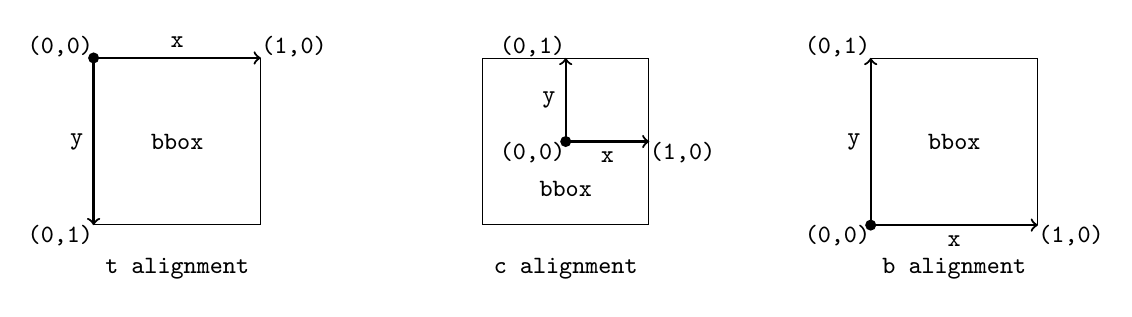
\begin{tikzpicture}[box/.style={draw, minimum width=6em, minimum height=6em},font={\tt\small}]
    \node[box] (t) {bbox};
    \node[below=2ex] at (t.south) {\ttx{t} alignment};
    \begin{scope}[shift=(t.north west), x=(t.north east), y=(t.south west)]
      \fill (0,0) circle (2pt);
      \draw[thick,->] (0,0) -- (1,0) node [midway,above] {x};
      \draw[thick,->] (0,0) -- (0,1) node [midway,left] {y};
      \node at (0,0) [above left,inner sep=0pt] {(0,0)};
      \node at (0,1) [below left,inner sep=0pt] {(0,1)};
      \node at (1,0) [above right,inner sep=0pt] {(1,0)};
    \end{scope}

    \node[box, right=8em, text height=4em] at (t.east) (c) {bbox};
    \node[below=2ex] at (c.south) {\ttx{c} alignment};
    \begin{scope}[shift=(c), x=(c.east), y=(c.north)]
      \fill (0,0) circle (2pt);
      \draw[thick,->] (0,0) -- (1,0) node [midway,below] {x};
      \draw[thick,->] (0,0) -- (0,1) node [midway,left] {y};
      \node at (0,0) [below left,inner sep=0pt] {(0,0)};
      \node at (0,1) [above left, inner sep=0pt] {(0,1)};
      \node at (1,0) [below right,inner sep=0pt] {(1,0)};
    \end{scope}

    \node[box, right=8em] at (c.east) (b) {bbox};
    \node[below=2ex] at (b.south) {\ttx{b} alignment};
    \begin{scope}[shift=(b.south west), x=(b.south east), y=(b.north west)]
      \fill (0,0) circle (2pt);
      \draw[thick,->] (0,0) -- (1,0) node [midway,below] {x};
      \draw[thick,->] (0,0) -- (0,1) node [midway,left] {y};
      \node at (0,0) [below left,inner sep=0pt] {(0,0)};
      \node at (0,1) [above left,inner sep=0pt] {(0,1)};
      \node at (1,0) [below right,inner sep=0pt] {(1,0)};
    \end{scope}
  \end{tikzpicture}
  \end{center}
  \end{commandalt}
  
  \begin{commandalt}[layer grid (layer scope option)]{{layer grid}\opt{=\meta{options}}}{}
    Draw a grid within the current \ttx{layer xy} coordinates.  By default the
    grid fills the layer.  Fine minor grid lines are 0.1 units apart. and
    heavier major grid lines are placed at full units.  The default appearance
    is taken from the \TikZ\ \ttx{help lines} style, with major lines drawn
    \ttx{thick}.  The appearance and grid parameters can be changed using
    \ometa{options}, which may include the following special keys:
    \begin{description}
    \item[\tt min=\meta{value}] The minimum coordinate of the grid; \meta{value}
      should be a number that applies to both \ttx x and \ttx y dimensions
      (default=0 for \ttx t and \ttx b aligned coordinates, or -1 for \ttx c).
    \item[\tt max=\meta{value}] The maximum coordinate of the grid; \meta{value}
      should be a number that applies to both \ttx x and \ttx y dimensions (default=1).
    \item[\tt spaced=\meta{value}] the spacing between grid lines (default = 0.1 for
      minor, or 1 for major).
    \item[\tt minor=\marg{options}] options for the minor grid only (may include
      \ttx{min\OR max\OR spaced}).
    \item[\tt major=\marg{options}] options for the major grid only (may include
      \ttx{min\OR max\OR spaced}).
    \end{description}
  \end{commandalt}
\end{envwithcontents}
\poppdfbookmark


\begin{environment}{{layers<>}
    \oarg{parameter spec}\marg{code}\optsarg{default specification}}
  This is a synonym for |\begin{incrementallayers} ... \end{incrementallayers}|.
\end{environment}



\subsection{Synchronising incremental environments}\label{sec:envs:synch}

After an incremental environment has been defined, the special label
\ttx{next\,+} evaluates to the increment associated with the next \ttc\next: or,
more precisely, to the smallest \ttx{/next\,\meta{n}/} that is strictly greater
than the current increment or to 0 if none are larger.  This label can be used
to easily synchronise later incremental environments to a first one, even if
each \ttc\next\ step involves multiple increments.  \example
\begin{verbatim}
  \begin{<>}
  \next first line \onslide<+->{with an addendum}\\
  \next second line\\
  \end{<>}

  \resetincr % ensure currentincr is less than /next 1/
  \begin{<>}[<!/next +/->]
  \next match the first line on slide \incrref{next 1}\\
  \next match the second line on slide \incrref{next 2}\\
  \next match the second line on slide \incrref{next +}\\
  \end{<>}
\end{verbatim}
The reset specification in \ttx{<!/next +/->} is necessary to advance the current
increment.
%
The values of \ttx{next\,\meta{n}} are redefined in the second environment, but
mostly to the same values as in the first.  The exception in this example is
\ttx{next\,0} which will be set to 1 (by the \cmd\resetincr) regardless of its
value in the first environment.  As a side effect, this ensures that \ttx{/next
  +/} at the first \ttc\next\ call evaluates to \ttx{/next 1/} rather than
\ttx{/next 0/}.

It is possible to wrap an \ttx{itemize} environment within an incremental one to
provide a similar functionality, albeit with warnings discussed below.
\example
\begin{verbatim}
  \begin{<>}\begin{itemize}
  \next\item<.-> first item \item with an addendum\\
  \next\item<.-> second item\\
  \end{itemize}\end{<>}

  \resetincr[/next 0/] % ensure currentincr is less than /next 1/
  \begin{itemize}[<!/next +/->]
  \item match the first item on slide \incrref{next 1}\\
  \item match the second item on slide \incrref{next 2}\\
  \item match the second item on slide \incrref{next +}\\
  \end{itemize}
\end{verbatim}
The explicit \ttx{<.->} specifications in the first \ttx{itemize} are needed
because the incremental environment sets the default spec to \ttx{<+->}, and so
would otherwise cause each \ttc\item\ to introduce a new increment.  It is not
possible to set separate default specs for the incremental and \ttx{itemize}
environments when both are used explicitly.  Thus, the addendum
\ttc\item\ inherits the \ttx{<+->} default.

The second \ttx{itemize} does not need to be wrapped within an incremental
environment.  It simply accesses the labels defined in the first.

Note that both the \ttx{incremental} and \ttx{itemize} environments group the
contents of \ttc\next\ or \ttc\item\ commands within environments.  it is thus
surprising that the interleaved construct works at all.  There are cases where
it will fail.  In general, when using |\next\item| it is best to have display
(or uncover) control determined by the \ttc\next\ command, but appearance (such
as alerts) determined by the \ttc\item.  

A shorthand environment is available, which adds the capability to define
separate default specifications for \ttc\next\ and \ttc\item\ calls.  However,
this does not resolve the fragility of the interleaving.

\begin{envwithcontents}{{incrementalitemize}\optsarg{default
      specification}\opt{\tt[\sarg{next item default}\&\sarg{separate item default}\ttx]}}
  {\item \hskip1em \osarg{pre-next specification} \opt{\meta{pre-next contents}}
    \item \ttx{\string\next}\osarg{next specification}
    \item \hskip1em \meta{next contents}
    \item \ttx{\string\item}\osarg{item specification}
    \item \hskip1em \meta{item contents}
    \item \hskip2em $\vdots$
  }
  This environment is similar to 
\begin{verbatim}
  \begin{docmd<>}[0]{\item<.->}
  \begin{itemize}
  \next<next specification> next contents 
  \item<item specification> item contents        
  ...
  \end{itemize}
  \end{docmd<>}
\end{verbatim}
  Each \ttc\next\ creates an \ttc\item\, by default displayed from the increment
  in effect after the \ttc\next.  It also increments the \ttx{next} counter and
  defines a corresponding \ttx{next\,\meta{n}} label.  An explicit
  \ttc\item\ uses the same default specification as \ttc\next\ (which itself
  defaults to \ttx{<+->} in incremental environments), but does not set the
  next-related counter or label.

  The second optional argument (which must follow the first) makes it possible
  to change the default overlay behaviour of the \ttc\item s.  It can contain
  one or two specifications, separated by an \& symbol.  The first applies to
  the implicit \ttc\item\ commands generated by each \ttc\next.  The second, if
  present, applies to any explicit \ttc\item s.  If absent, it is set to the
  overall default specification.  The default values if no optional arguments
  are given are |[<+->][<.->&<~>]|.

  
  
  Note that any \meta{pre-next contents} cannot generate typeset text, as this
  would precede the first \ttc\item\ command.
\end{envwithcontents}
\begin{environment}{{itemize<>}\optsarg{default specification}}
  This is a synonym for |\begin{incrementalitemize} ... \end{incrementalitemize}|.
\end{environment}


\section{Incremental alignment environments}\label{sec:align}
\locsection{Alignment environments}

Standard \LaTeX\ alignment environments including \ttx{tabular} and the \ttx{align}
and \ttx{align*} environments from the \ttx{amsmath} package are not ordinarily
increment-aware.  The current package introduces a partial fix for this,
although their are remaining fragilities that may need to be worked around.  It
is possible to make an increment-aware version of any alignment environment
using \cmd\CreateIncrementalAlignmentEnvironment\ as described below.  A few such
environments are defined automatically when \beamincr\ is loaded and these are
described first, thus illustrating the behaviour once an increment-aware
environment has been created.

\subsection{Automatically defined incremental alignment environments}\label{sec:align:auto}

\vskip 2ex
\noindent
The following two environments are equivalent:
% \begin{environment}{{incrementalalign}\opt{\ttx{[<}\meta{spec1}\ttx{>\&<}\meta{spec2}\ttx{>\& ...]}}}
% \end{environment}
% \begin{environment}{{align<>}\opt{\ttx{[<}\meta{spec1}\ttx{>\&<}\meta{spec2}\ttx{>\& ...]}}}
% \end{environment}
\begin{environment}{{incrementalalign*}\opt{\ttx{[<\meta{spec1}>\&<\meta{spec2}>\&...]}}}
\end{environment}
\vskip -2ex
\begin{environment}{{align*<>}\opt{\ttx{[<\meta{spec1}>\&<\meta{spec2}>\&...]}}}
  Each pre-processes the input to \ttx{align*}, placing an |\action<>{}| command
  around each field, defined as the material appearing between successive |&|,
  |\\| or end environment tokens.  By default, the first field on a line is
  called with |\action<+->{}|, and up to 7 remaining ones with |\action<.->{}|.
  This has the effect of displaying a full line at a time, unless it has more
  than 8 fields.  The optional argument makes it possible to change this
  behaviour to \ttc{\action<\ometa{spec1}>}, \ttc{\action<\ometa{spec2}>},
  etc.\ with the sequence of specifications reset to \ttx{<\ometa{spec1}>} at
  the beginning of every line. If there are fewer specifications in the default
  than fields on a single line, then the sequence is repeated.  The default
  specification values can be changed by calling
  \cmd\setincrementalenvspec\ttx{\{align*\}\{<\meta{new default}>\}} or similar.

  The default specification for a single field can be overridden by placing a
  field-specific specification in \ttx{<>} at its start.  This means that a
  leading \ttx< in the field contents itself must be protected, e.g.\ by preceding
  it with |{}|.

  The use of \ttc\action\ means that \beamer\ will interpret both standard
  \ttx{action@\meta{increment}} actions and implicit ones such as \ttx!-prefixed
  increment resets, \ttx= label assignments or |~|\meta{range} default
  specification.
\example
\begin{verbatim}
  \begin{align*<>}[<+->&<.->] % increment after every two &s
    x\incrlabel{x} &= y  &  1 &{}< 2 \\
    </x/-> x^2 &= y^2    &  <!/x/-> e^{i\pi} &<+->= -1 \\
    \sum_n f(n) &<.-|alert@.> \to \int f(x) dx
  \end{align*<>}
\end{verbatim}
    
    The pre-processor is not able to distinguish between the |&| alignment
    characters that apply to the containing environment and any that appear
    within enclosed environments, such as \ttx{array}.  Thus, any such
    environments must be protected.  The simplest approach is just to add extra
    braces to group the enclose environment at a lower level.  Alternatively,
    the environment can be defined within a token register or a protected macro.
    It is still possible to use increments within the environments: these are
    processed sequentially with those in the containing |align| environment,
    respecting increment labels, resets etc.

    \example
\begin{verbatim}
  % using grouping
  \newtoks\mymatrix
  \begin{align<>}
    \incrlabel{mat}{\begin{pmatrix} 1 & 2 \\ \alt<+->{3}{2} & 4 \\ \end{pmatrix}}\resetincr[/mat/]
    & \text{is \only<+->{not }singular}
  \end{align<>}

  % using \protected
  \protected\def\mymatrix{\begin{pmatrix} 1 & 2 \\ \alt<+->{3}{2} & 4 \\ \end{pmatrix}}
  \begin{align<>}
    \incrlabel{mat}\mymatrix \resetincr[/mat/]& \text{is \only<+->{not }singular}
  \end{align<>}

  % using token registers
  \newtoks\mymatrix
  \mymatrix={\begin{pmatrix} 1 & 2 \\ \alt<+->{3}{2} & 4 \\ \end{pmatrix}}
  \begin{align<>}
    \incrlabel{mat}\the\mymatrix \resetincr[/mat/]& \text{is \only<+->{not }singular}
  \end{align<>}

\end{verbatim}
    It may be wise to put any \ttc\newtoks\ declaration outside the frame so as not
    to consume more of \TeX's resources than needed.  

    \ttc\intertext\ lines must be terminated with |\\|.  By default they will be
    grouped within the action call of the last field of the preceding line.
    This behaviour can be changed by inserting a |\\| between that field and the
    \ttc\intertext.  By default, both |\\|s will add extra vertical space (and an
    equation number in non-starred variants).  These can be avoided by using
    a form like |\nonumber\\[-3ex]| instead.

    The \ttx{amsmath} \ttc\tag\ command is processed in such a way that it
    cannot easily be made overlay aware.  Any \ttc\tag s will appear on any slides
    where the overall environment is uncovered, even if no fields have appeared.
    However, an alternative \cmd\eqtag\ is defined.  See \cref{sec:align:eqnum}.
    
\end{environment}
%
\begin{environment}{{incrementalgather*}\optsarg{default spec}}
\end{environment}
\vskip -2ex
\begin{environment}{{gather*<>}\optsarg{default spec}}
These incremental forms are also created when \beamincr\ is loaded, with similar
behaviour to the incremental \ttx{align*} environments described above.
Although these contain only one field per line, automatic access to \beamer\ and
\beamincr\ actions as these lines are processed can be useful.  By default, they
uncover equations a line at a time (using \ttx{<+->}).
\end{environment}


\begin{environment}{{incrementaltabular}\oarg{pos}\marg{cols}\opt{\tt[<\meta{spec1}>\&<\meta{spec2}>\&...]}}
\end{environment}
\vskip -2ex
\begin{environment}{{tabular<>}\oarg{pos}\marg{cols}\opt{\tt[<\meta{spec1}>\&<\meta{spec2}>\&...]}}
  These provide increment-aware versions of the standard \LaTeX\ \ttx{tabular}
  environment.  By default, the entire table is uncovered on the current
  increment (using \ttx{<.->}), but this behaviour can be altered by changing
  the default specification when called, or by using
  \cmd\setincrementalenvspec\ as described below.  It may also be desirable to
  uncover entries column-by-column.  This effect can be achieved using increment
  labels.  \example
\begin{verbatim}
\begin{tabular<>}{cccc}[</col1-/>&</col2-/>&</col3-/>&</col4-/>]
  <=(1)>/col1/\bf fruit & <=(2)>/col2/\bf colour  
      & <=(3)>/col3/\bf climate & <=(4)>/col4/\bf family \\[1ex]
  Apple & green & cool & pome \\
  Peach & yellow & warm & drupe \\
  Plum & purple & cool & drupe \\
  Orange & orange & hot & citrus \\
\end{tabular<>}  
\end{verbatim}
\end{environment}

\begin{environment}{{incrementaltabular*}\oarg{pos}\marg{width}\marg{cols}\opt{\tt[<\meta{spec1}>\&<\meta{spec2}>\& ...]}}
\end{environment}
\vskip -2ex
\begin{environment}{{tabular*<>}\oarg{pos}\marg{width}\marg{cols}\opt{\tt[<\meta{spec1}>\&<\meta{spec2}>\& ...]}}
  These forms add the \meta{width} argument of \LaTeX's \ttx{tabular*} environment.
\end{environment}

\subsection{Creating new incremental alignment environments}\label{sec:align:new}

\begin{command}{{\CreateIncrementalAlignmentEnvironment}\rlap{\marg{name}\oarg{Nopts}\marg{Nreqs}%
    \opt{\ttx{[<\meta{default spec}>]\oarg{base}}}}}
  {create \ttx{incremental\meta{name}} and \ttx{\meta{name}<>} variants of
    \meta{name} [or \ometa{base}] environment}
    
  Create an increment-aware version of an alignment environment.  Unless a
  different \meta{base} environment is specified in the final argument, the new
  environment is based on an existing one of the same \meta{name}.  This
  existing environment should process its contents in fields demarcated by |&|
  and/or |\\| tokens.  The arguments \meta{Nopts} and \meta{Nreqs} specify the
  numbers of optional and required arguments the base environment expects.  If
  \meta{Nopts} is omitted it is taken to be 0.  \meta{Nreqs} must be specified,
  but can be 0.  If the \meta{default specification} is omitted it is set to
  \ttx{<.->}, thus displaying the environment contents at the prevailing increment
  number in the frame.

  The new environment can be accessed using either of the names
  \ttx{incremental\meta{name}} or \ttx{\meta{name}<>}.
\end{command}

\subsection{Manipulating default behaviour}\label{sec:align:defaults}

\begin{command}{{\useincrementalenv}\marg{name}}%
  {make  subsequent uses of the \meta{name} call the incremental environment \ttx{\meta{name}<>}}
  Make all subsequent uses of the \meta{name} environment call the incremental
  version.  The incremental version must already have been created.
  \example
\begin{verbatim}
\useincrementalenv{align*}
\begin{align*}[<+->]
  % this is an incremental environment
\end{align*}
\end{verbatim}
  The specified \meta{name} must match the \emph{name} of the base environment
  (i.e., the first argument to \cmd\CreateIncrementalAlignmentEnvironment), whether
  or not this is the same as its base.
  %
\example
\begin{verbatim}
\CreateIncrementalAlignmentEnvironment{foo}{0}[<.->][bar]
\begin{foo}
  % error -- environment is accessible as incrementalfoo or foo<>
\end{foo}
\useincrementalenv{foo}
\begin{foo}
  % evokes the incremental version of bar
\end{foo}
\end{verbatim}
\end{command}

\begin{command}{{\usenonincrementalenv}\marg{name}}%
  {make subsequent uses of \meta{name} call non-incremental \meta{base} environment defined at creation}
  Make subsequent uses of the \meta{name} environment refer to the
  non-incremental version.  If the name and base specified at creation were the
  same, this restores the normal behaviour of the \meta{name} environment.  If a
  different base environment was specified at creation, this creates a new
  \meta{name} environment that is synonymous with the base.  \example
\begin{verbatim}
\CreateIncrementalAlignmentEnvironment{foo}{0}[<.->][bar]
\begin{foo}
  % error -- environment is accessible as incrementalfoo or foo<>
\end{foo}
\usenonincrementalenv{foo}
\begin{foo}
  % evokes the original version of bar
\end{foo}
\end{verbatim}
\end{command}


\begin{command}{{\setincrementalenvspec}\marg{name}\marg{default
      specification}}%
  {set the default specification for incremental \meta{name} environments }
  Set the default specification for incremental environments of type \meta{name}.
\end{command}


\subsection{Equation numbering}\label{sec:align:eqnum}

Unfortunately, the \ttx{amsmath} \ttc\tag\ command, used for equation numbering, is
processed in such a way that it cannot easily be made overlay aware.  Any
\ttc\tag{}s will appear on any slides where the overall environment is uncovered,
even if no fields have appeared.  This is also the case with automatic
numbering.  Thus if defined using
\begin{verbatim}
  \CreateIncrementalAlignmentEnvironment{gather}{0}[<+->]
\end{verbatim}
the \ttx{gather<>} environment will also generate all equation numbers whenever
the environment as a whole is uncovered, regardless of the status of the
relevant fields.  In principle, this behaviour could be partially addressed
using a technique discussed in the \beamer\ manual Howtos, but this requires
some additional hackery.

Instead, beamincr provides an increment-aware version of \ttc\tag\ and of
automatic equation numbering.
\begin{command}{\eqtag\sarg{overlay spec}\marg{tag}}%
  {place \meta{tag} on slides that match \meta{overlay spec}}
  Place \meta{tag} on slides that match \meta{overlay spec}.  
\end{command}
\begin{command}{\eqnum\sarg{overlay spec}}
  {place current equation number on slides that match \meta{overlay spec}, and increment}
%
  Place the current equation number (as \ttc\theequation) on slides that match
  \meta{overlay spec}, and then increment it.
\end{command}

The second form can be used as an action.
\begin{commandalt}[<eqnum@>]{{<eqnum@}\meta{range}\contcmd{>}}{}
  Place the current equation number (as \ttc\theequation) on slides in
  \meta{range}, and then increment it.
  \example
\begin{verbatim}
\begin{align*}[<+-|eqnum@+->&<.->]
  e^{\pi i} &= -1 \\
  \sqrt[3]{1} &= e^{2\pi i/3}
\end{align*}
\end{verbatim}
numbers equation as it is uncovered.  
\end{commandalt}

In principle, this method can be used to create automatic numbering forms of the
amsmath environments:
\begin{verbatim}
\CreateIncrementalAlignmentEnvironment{gather}{0}[<+-|eqnum@+->][gather*]
\begin{gather<>}
  % equations will be numbered, with numbers uncovered with the rest of the line
\end{gather<>}
\end{verbatim}
Such environments are not created automatically, as the user should be aware of
two traps.  First, if a default specification is given to |\begin{gather<>}|,
the environment will revert to unnumbered unless the appropriate \ttx{eqnum}
action or commands are provided.  Second, a call to
\cmd\usenonincrementalenv|{gather}| will make \ttx{gather} a synonym for
\ttx{gather*}.  At this point, there would be no easy way to restore \ttx{gather} to
its original behaviour.  You have been warned.


\section{Directing attention}\label{sec:attention}
\locsection{Directing attention}

\subsection{Alerts}

\begin{command}{\alerts\sarg{overlay spec}\marg{argument contents}}
  {activate \ttc{\alert*} commands in \meta{argument contents} on \meta{overlay spec}}
  %
  Activate any \cmd{\alert*} commands in \meta{argument contents} on the
  overlays indicated by \meta{overlay spec}.
\end{command}

\begin{commandalt}[<alerts@>]{{<alerts@}\meta{range}\contcmd>}{}
  This is the action equivalent of \cmd\alerts.
\end{commandalt}

\begin{command}{{\alert*}\marg{argument}}%
  {alert \meta{argument} when activated}
  %
  Executes \ttc\alert\marg{argument} if an enclosing \cmd\alerts\ command or
  action is active.  Otherwise \meta{argument} is displayed unalerted.
\end{command}



\subsection{Pointers}

\begin{command}{\point\osarg{overlay spec}\marg{contents}}%
  {insert pointer as appropriate, and activate \ttc{\point*} commands in \meta{range}}
  In normal text, insert a pointer before \meta{contents} on the specified
  slides.  If \meta{contents} includes any \cmd{\point*} commands, pointers are
  inserted at the locations of these commands at the same time.

  If called within a \TikZ\ picture, the \ttc\point\ command does not insert a
  pointer itself.  Instead, any pointer defined by the \ttx{pointer} option
  to any nodes in \meta{contents} is activated.  See the description of
  \ttx{pointer} below.
\end{command}

\begin{commandalt}[<point@>]{{<point@}\meta{range}\contcmd>}{}
  The action form of \cmd\point\ can be used in all contexts where an action
  specification is valid.  Its behaviour around normal text or \TikZ\ code is as
  above.  In \ttx{itemize} environments it replaces the default item label with
  the pointer\footnote{Although if the \ttx{itemize} is nested within an
  \ttx{enumerate}, it inherits the \ttx{enumerate} behaviour.}.  In
  \ttx{enumerate} environments it prepends the pointer to the default label.  In
  other list environments, or when the label is set explicitly as an optional
  argument to \ttc\item, it has no direct effect.  However any \cmd{\point*}
  commands in the item label or text are activated.
\end{commandalt}

\begin{commandalt}[<pointers@>]{{<pointers@}\meta{range}\contcmd>}{}
  This action activates \cmd{\point*} commands in the argument contents, but
  does not insert a pointer.
\end{commandalt}

\begin{command}{{\point*}\oarg{options}\opt{\marg{contents}}}
  {insert a pointer when activated (possibly using a \TikZ\ node around
    \ometa{contents})}
  %
  If the command is not followed by a |[| or |{| character, insert a pointer
      when an enclosing \cmd\point\ command or action is active.

  If followed by an argument in |[]| or |{}|, and if \TikZ\ is loaded, call
  \cmd\pointtonode\ as described below.  If \TikZ\ is \emph{not} loaded a normal
  pointer is inserted as in the no-argument form, any options are ignored, and
  the contents is copied to the output.
\end{command}

\begin{commandalt}[pointer (tikz option)]{{tikz option: pointer}\opt{=}\oarg{pointer node options}\opt{\meta{angle}}}{}
  This is a \TikZ\ option that can be passed to a \ttx{node} to insert a
  pointer drawn towards the node whenever an enclosing \cmd\point\ command or
  action is active.  If an \meta{angle} is specified, the pointer is drawn
  towards the corresponding point on the node boundary; this can be specified as
  a numerical angle or a direction like \ttx{north}.  The default angle is
  \ttx{west} or \ttx{180}, so that the pointer points to the node from the
  left.  The pointer itself is drawn within a node: this behaviour is very
  similar to the regular \TikZ\ node \ttx{label} option, except that the
  pointer node is automatically sloped so as to point inwards.

  The current implementation does not work well with \ttx{coordinate}s.  The
  alternative \ttx{pointer coordinate} style creates an empty circular node
  of 0.1pt size, which is broadly equivalent.

  If \meta{pointer node options} are specified (generally requiring braces
  around the entire option value to protect \TikZ's option parsing from seeing
  the |[]|s) these are passed to the pointer node.  A few options may be
  particularly useful:
  \begin{description}
    \item[\tt pos=\meta{scale}] adjusts the placement of the pointer as a
      fraction of the distance from the target node centre to its boundary.  The
      default is 1.0.  This option is unlikely to be useful when the target is a
      \ttx{pointer coordinate}.
    \item[\tt pointer sep=\meta{dimen}] adds \meta{dimen} to the distance of the
      pointer from the target node.
    \item[\tt rotate=\meta{angle}] rotates the pointer relative to its initial
      angle.
  \end{description}
\end{commandalt}


\begin{command}{\pointtonode\oarg{{\tt pointer} options}\marg{contents}}
  {insert a pointer to a \TikZ\  node when activated}
  If \TikZ\ is loaded, this is shorthand for
\begin{verbatim}
  \tikz[baseline]\node[anchor=base,text height=1.5ex,inner sep=0pt,pointer={#1}]{#2};
\end{verbatim}
The spacing adjustments ensure that the contents in the node are printed in
alignment with the surrounding text, and that pointers to an empty node appear
at a similar height to those inserted by \cmd\point\ or \cmd{\point*}.  The
availability of \meta{{\tt pointer} options} provides flexibility in the pointer
placement.

If \TikZ\ is not loaded, this is the equivalent of \cmd{\point*}\marg{contents},
ignoring any options given.
\end{command}

\begin{command}{\usepointer\oarg{inactive glyph}\marg{pointer glyph}}
  {set the pointer glyph}
  %
  Use \meta{pointer glyph} for subsequent pointers in the current group.  If the
  optional argument is absent, then the pointer is replaced by a phantom of the
  same size when inactive (the size only matters if \cmd\useuncoverpointer\ is
  active).  If it is given, then inactive pointers are replaced by
  \meta{inactive glyph} (which may be empty).
  %
  \example
\begin{verbatim}
\usepointer{\raisebox{0.3ex}{\alert{$\blacktriangleright$}}} % the default
\usepointer{\raisebox{-0.4ex}{\alert{\HandRight}}} % requires \usepackage{bbding}
\end{verbatim}
Note that some adjustment of the vertical placement, as in these examples, may
be necessary to align the pointer appropriately with the text.

The effect of this command is local to the containing group. 

The pointer appearance should really be controlled through \beamer's template
mechanism, but that's a project for another day.
\end{command}

\begin{command}{\useoverprintpointer}
  {pointer glyphs take up no space and print on top of existing text}
  Print subsequent pointers (and any inactive glyphs) in the current group
  \emph{over} existing material, without reserving any space for them
  (internally, they set within a zero-width box). This is the default, and
  avoids the dilemma of either leaving blank spaces for inactive pointers, or
  having text rearrange when the pointer appears.

  The effect of this command is local to the containing group. 
\end{command}

\begin{command}{\useuncoverpointer}
  {reserve space for pointer glyphs}
  Set subsequent pointers and any inactive glyph in the current group as normal
  text, taking up space on the page.  If no inactive glyph has been specified,
  the effect is to leave a blank space when the pointer is inactive, much like
  the effect of the \ttc\uncover\ or \ttc\onslide\ commands.  If the inactive glyph is
  set to the empty string, there is no blank space, but surrounding text is
  rearranged to make room for the pointer when it becomes active.

  The effect of this command is local to the containing group. 
\end{command}



\subsection{Graphical alerts}\label{sec:attention:glerts}

If \TikZ\ is loaded, \beamincr\ defines various styles of graphical alerts or
\ttx{glerts}, and provides a facility to define more.  The argument to be
alerted is set within an inline \TikZ\ node with a tight bounding box, aligned
with the baseline of the surrounding line of text.  A second node or associated
path is used to add the graphical embellishment. (More details of the
construction are given in \cref{sec:attention:glerts:refining}.)  Glerts can be
used to draw attention at specific increments, or simply to highlight material
on the slide in a static fashion.

\subsubsection{Glert commands}\label{sec:attention:glerts:cmds}

The following commands are used to insert and control the activation of glerts.

\begin{command}{\useglert\tt\{\meta{style}$_1$\opt{=\meta{options}},
    \opt{\meta{style}$_2$=\meta{options}}, \oarg{further options}\}}
  {set style and options for future glerts}
  %
  Set one or more glert styles to be applied to subsequent \ttc{\glert[*]} calls
  or actions, unless they define a style locally.  For a discussion of the
  \ometa{further options}, see \cref{sec:attention:glerts:refining}.
\end{command}

\begin{command}{\addglert\tt\{\meta{style}$_1$\opt{=\meta{options}},
    \opt{\meta{style}$_2$=\meta{options}}, \oarg{further options}\}}
  {add style and options for future glerts}
  %
  Append one or more glert styles to the current set, to be applied to subsequent
  \ttc{\glert[*]} calls or actions, unless they define a style locally.  
\end{command}


\begin{command}{\glert\sarg{overlay spec}\oarg{options}\marg{argument contents}}
  {apply a graphical alert to \meta{argument contents} on \meta{overlay spec}}
  %
  Apply a graphical alert to \meta{argument contents} on \meta{overlay spec}.
  The style of the alert may be set in \ometa{options} using the same syntax as
  in \cmd\useglert.  When inactive, \meta{argument contents} is displayed
  unalerted within a \TikZ\ node.
\end{command}

\begin{command}{{\glert*}\oarg{options}\marg{argument contents}}%
  {apply a graphical alert to \meta{argument contents} when activated}
  %
  Executes \ttc\glert\oarg{options}\marg{argument contents}, with the active or
  inactive state determind by the status of any enclosing \cmd\glerts\ command
  or action.  If there is no such command, then the glert is always inactive.
\end{command}

\begin{command}{\glerts\sarg{overlay spec}\marg{argument contents}}
  {activate \ttc{\glert*} commands in \meta{argument contents} on \meta{overlay spec}}
  %
  Activate any \cmd{\glert*} commands within \meta{argument contents} on the
  overlays indicated by \meta{overlay spec}.
\end{command}

\begin{commandalt}[<glerts@>]{{<glerts@}\meta{range}\contcmd>}{}
  This is the action equivalent of \cmd\glerts.
\end{commandalt}


\subsubsection{Glerts and modes}\label{sec:attention:glerts:modes}

Ordinarily, glerts remain inactive in all except \ttx{beamer} mode.  To include
an active glert in (say) \ttx{handout} mode, include the mode spec
\ttx{<handout>} or \ttx{<handout:*>} within the \meta{spec} passed to
\cmd\glert.  The same options can can be included in the spec of an explicit
\cmd\glerts\ command.  To activate \cmd{\glert*}s implicitly from an enclosing
action, use \ttx{<handout:glerts@*>}.

Alternatively, when using \cmd\handoutframe, specific overlays can be included
within the handout (or other mode) output rendered as they would be in
\ttx{beamer} mode.


\subsubsection{Built-in glert styles}\label{sec:attention:glerts:builtin}

A few \ttx{glert} styles are predefined.  Each displays the text in the same
style as the surrounding material when inactive.  Their actions when activated
are as follows.
  \begin{commandalt}[null (glert style)]{{glert style: null}}
    {do nothing, even when activated}
    Do nothing, even when activated.
  \end{commandalt}

\begin{commandalt}[alert (glert style)]{{glert style: alert}=\ometa{color, \dots}}
  {display text in red or \ometa{color}}
  Display text in red or \ometa{color} (like the standard \ttc\alert).  This is
  the default glert style.  
\end{commandalt}

\begin{commandalt}[box (glert style)]{{glert style: box}=\ometa{color, \dots}}
    {draw a rectangular frame around the text in red or \ometa{color}}
    Draw a rectangular frame around the text in red or \ometa{color}.
\end{commandalt}

\begin{commandalt}[ellipse (glert style)]{{glert style: ellipse}=\ometa{color, \dots}} 
  {draw an ellipse around the text in red or  \ometa{color}}
  Draw an ellipse around the text in red or  \ometa{color}.
\end{commandalt}

\begin{commandalt}[uline (glert style)]{{glert style: uline}=\ometa{line options}}
  {underline the text}
  Underline the text.  The appearance of the line can be altered with standard
  \TikZ\ line options.  The default is red and  ``very thick''.
\end{commandalt}

\begin{commandalt}[sout (glert style)]{{glert style: sout}=\ometa{angle, line  options}}
  {strikeout the text with a horizontal (or at \ometa{angle} from horizontal) line} 
  Strikeout the text by placing a horizontal line (or line tilted by
  \ometa{angle} from horizontal) through it.  The \meta{angle} may be a
  direction keyword such as \ttx{north east}.  The appearance of the line can be
  altered with standard \TikZ\ line options.  The default line is red and ``very
  thick''.
\end{commandalt}

\begin{commandalt}[xout (glert style)]{{glert style: xout}=\ometa{angle, line options}}
  {cross out text with an X shape joining the node corners, or at \ometa{angle}
    from horizontal}
  A version of \ttx{sout} that adds a
  second line flipped vertically from the first, creating an X shape.  The
  default behaviour is to join opposite corners of the containing node (equivalent to
  \meta{angle}=\ttx{north east}), otherwise they are drawn $\pm$\meta{angle}
  from horizontal.  The appearance of the lines can be altered with standard
  \TikZ\ line options.  The default lines are red and ``very thick''.
\end{commandalt}

\begin{commandalt}[highlight (glert style)]{{glert style: highlight}=\ometa{color, \dots}}
  {fill a background box with partly transparent red or \ometa{color}}
  Fill a background box with partly transparent
  red or \ometa{color}, much as a highlighter would on paper.
\end{commandalt}

\begin{commandalt}[spotlight (glert style)]{{glert style: spotlight}=\ometa{color, \dots}}
  {draw a fading ellipse underneath the text in partly transparent red or \ometa{color}}
  Draw a fading ellipse underneath the text in partly transparent red or \ometa{color}.
\end{commandalt}

\begin{commandalt}[connect (glert style)]{{glert style: connect}=\{\oarg{to options} \meta{target}\}}
  {draw a [red, very thick, double-headed arrow] line to \meta{target}
    coordinate}
  Draw a [red, very thick, double-headed arrow] line to the \TikZ\ coordinate
  \meta{target}.  This could be a \ttx{(\meta{glert name})} (see
  \cref{sec:attention:glerts:names}).  If it is the name of a node in another
  \TikZ\ picture, that picture must have the \ttx{remember picture} option set;
  this is always the case for glerts.

  The \ometa{to options} can be used to modify the shape of the path.  The style
  of the line can be changed by specifying \ttx{path=\marg{options}} within the
  \ometa{further options} of the \cmd\glert\ttx{[*]} command.
\end{commandalt}

\begin{commandalt}[label (glert style)]{{glert style: label}=\{\oarg{path options}\meta{angle}:\oarg{label node
    options}\meta{label text}\}}
  {place a node containing \meta{label text} at \meta{angle} from the glert node}
  %
  Place a label near the glert node.  This is similar to the \TikZ\ label and
  pin options, but allows more automated placement and orientation control
  (beside, of course, being controlled by the \cmd\glert\ incremental system).

  The  \meta{path options} may include:
  \begin{description}\topsep=0pt
  \item[\tt pos=\meta{scale}] Scale separation from glert node centre in
    proportion to the glert node ``radius''.  This is similar to the
    \TikZ\ \ttx{pos} option for placing a node on a line, where the line in
    question extends from the centre of the glert node to its border.  Thus,
    setting \ttx{pos=2} sets the glert label anchor twice as far from the glert
    node centre as its border in the direction \meta{angle}.

  \item[\tt sep=\meta{dimen}] Add \meta{dimen} to the separation from glert
    node.  If \meta{angle} is a keyword, \ttx{pos} moves along the corresponding
    direction defined by the glert node shape, whereas \ttx{sep} moves in the
    corresponding absolute direction (e.g. $45^\circ$ for \ttx{north east}).

  \item[\tt from=center\OR border\OR corner\OR\meta{coord}] Start the path
    defining a sloped label orientation (and a drawn path) from this location.

    The value \ttx{border} corresponds to the point on the border along the
    straight line between the glert node center and the label anchor (as
    calculated by the \TikZ\ node coordinate system: the coordinate is just set
    to \ttx{(\meta{glertnode})}), while \ttx{corner} refers to \ttx{(\meta{glert
        node}.\meta{angle})}.  These may differ if \meta{angle} is a keyword
    like \ttx{north east}.  It is also possible to specify an explicit
    coordinate (potentially defined in terms of \ttc\glertnode,
    \ttc\glertangle\ and other commands described in
    \cref{sec:attention:glerts:defining}).

    The value of \ttx{from} does not change the interpretation of \ttx{pos} or
    \ttx{sep}; they are always defined relative to the centre or corner as
    described above.  However, if \ttx{pos}=1 and \ttx{sep}=0pt (the defaults) then
    choosing \ttx{from=border\OR corner} creates a path of zero length, which
    cannot be used to orient the label.  Therefore \ttx{from=corner} increases
    the \ttx{sep} default to 0.1pt, while \ttx{from=border} increases the
    \ttx{pos} default to 1.001.

    Thus \\
    \hspace*{1em} \ttc{\glert[label=\{[from=corner, sloped]north west:\meta{label text}\}]}\marg{text}
    \\
    orients  the label at $135^\circ$, while
    \\
    \hspace*{1em} \ttc{\glert[label=\{[from=border, sloped]north west:\meta{label text}\}]}\marg{text}
    \\
    orients the label to point to the node centre.

  \item[\tt sloped\opt{=\meta{bool}}] Rotate the label to point towards \ttx{from}, by default
    flipping orientation as necessary to keep the text from being rendered
    upside down.

  \item[\tt allow upside down\opt{=\meta{bool}}]  Allow upside down text.  Should be given in
    \ttx{path options} to ensure that anchor orientation is correct.

  \item[\tt draw\opt{=\meta{color}}] Draw the path from \ttx{from} to the
    label.  Any additional line style options (or \ttx{path=\meta{options}} are
    applied to this path.
  \end{description}

  The \meta{label node options} may describe the appearance of the label, and
  its placement relative to the anchor point defined by the path.  Options
  include:
  \begin{description}
  \item[\ttx{anchor in}] Anchor to the east/west side closer to the glert node.
  \item[\ttx{anchor out}] Anchor to the east/west side farther from the glert node.
  \item[\ttx{inward}] Anchor to the east/west side father from the glert node,
    so that the label extends inward to the node from the anchor.
  \item[\ttx{outward}] Anchor to the east/west side closer to the glert node so
    that the label extends outward from the anchor, away from the node.
  \end{description}
    
\end{commandalt}
    
\begin{commandalt}[signal (glert style)]{{glert style: signal}=\{\oarg{path options}\meta{angle}:\oarg{signal node
      options}\meta{signal text}\}}
  {create a \ttx{label} using a \ttx{signal} node, with pointers determined by
    \ttx{\string|>\OR>>\OR>\string|\OR<\string|\OR<<\OR\string|<} option}
  Create a \ttx{label} using a \ttx{signal} node.  All the label options apply.
  In addition, the options \ttx{\string|>\OR>{}>\OR>\string|\OR<\string|\OR<{}<\OR\string|<}
  control the presence and orientation of signal pointers.  Right \ttx>s
  indicate pointers inwards to the glert node.
\end{commandalt}


\begin{commandalt}[callout (glert style)]{{glert style: callout}=\{\oarg{callout node options}\meta{angle}:\meta{callout text}\}}
  {draw a callout node containing \meta{callout text} pointing to the glert node from \meta{angle} (may be direction keyword)}
  Draw a callout node containing \meta{callout text} pointing to the glert node  from \meta{angle} (may be a direction keyword).

  The default callout is rectangular and placed at a centre-to-centre distance 2.5 times the glert
  node ``radius'': i.e., the distance from centre to edge in the direction of \meta{angle}.

  The \ometa{callout node options} can be used to change the callout appearance
  and placement.  

  Options can be set for all callouts using the \ttx{glert callout options}
  style.  Initially, this sets the defaults of \ttx{\{rectangle callout, draw,
    pos=2.5, sep=0pt\}}.
\end{commandalt}
In the \ometa{color, \dots} arguments, a colour name (as defined by the
\ttx{xcolor} package) can generally be followed by other line or node options
placed (along with the colour) in braces.  Such options should take precedence
over any default style, and over any options not grouped with the \meta{color}
argument.  The other ways to set options are described in
\cref{sec:attention:glerts:refining}.

Multiple styles can be used together.  It they set conflicting parameters
(e.g. \ttx{box} vs.\ \ttx{ellipse}) then the last in the calling sequence will
prevail.


\subsubsection{Naming glerts}\label{sec:attention:glerts:names}

The name of the glert node can be set within the \cmd\glert\ttx{[*]} options
with \ttx{node=\{name=\meta{name}\}}, or, more simply, \ttx{(\meta{name})}.  The
node can then be referenced by a \ttx{connect} glert, or from another
\TikZ\ picture (remembering to use \ttx{remember picture} and \ttx{overlay} as
appropriate).
 

\subsubsection{Glerts in math mode}\label{sec:attention:glerts:math}

Glert commands generally process math mode material transparently.  In
particular, there is no need to restore the math mode or style explicitly within
the argument as there would be with most other boxed commands.  However,
\TeX\ internals mean that to achieve this transparency, both the maths material
and associated glert drawing must be rendered internally four times (in each of
the four main maths styles), with only one rendering then being placed on the
output page.

Although the added compilation induced by this quirk is generally acceptable,
there is at least one context in which it creates a real difficulty.  If a named
glert is to be referenced (say, with the \ttx{connect} glert style), the same
name is associated with all four nodes in turn, ending with the
\ttc\scriptscriptstyle\ version.  If that version isn't the one used in the
final layout, then \TikZ\ treats the final named node as though it were in the
bottom left corner of the page.

To work around this issue \beamincr\ makes it possible to specify the correct
math style to be used within the glert options, thus removing the need for the
four versions.  The possible options are:  
\begin{description}
  \item[\tt displaystyle\OR\$\$] for \cmd\displaystyle
  \item[\tt textstyle\OR\$-] for \cmd\textstyle
  \item[\tt scriptstyle\OR\$\_] for \cmd\scriptstyle
  \item[\tt scriptscriptstyle\OR\$.\OR\$\_\_] for \cmd\scriptscriptstyle
\end{description}

\example
\begin{verbatim}
\begin{equation*}% simple, but slow and cannot access the names
\int_{\glert[(lo)]{-\infty}}^{\glert[(hi)]{+\infty}} e^{-i\omega t} d\omega = 2\pi\delta(t)
\end{equation*}

\begin{equation*}% contents rendered only once in the specified style
\int_{\glert[$_, (lo)]{-\infty}}^{\glert[$_, (hi)]{+\infty}}
       e^{-i\omega t} d\omega = 2\pi\delta(t)
\end{equation*}
\end{verbatim}

Note that \ttx{align} environments also set their contents multiple times (to
determine their sizes) and so glert naming doesn't work there either.  There's
no workaround for this at the moment.


\subsubsection{Glerts in \TikZ\ pictures}\label{sec:attention:glerts:tikz}

Glerts can be applied to nodes in \TikZ\ pictures by setting the options below.
In this use, no separate bounding box node is created.  Thus, the extent of the
node itself (including any glert-based modifications to the node) will
ordinarily contribute to the size of the picture.  However, any glert path
additions will not, and so may extend outside the picture bounding box.

\begin{commandalt}[glert (tikz option)]{{tikz option: glert}\ttx{=\{\sarg{overlay spec}\ometa{options}\}}}
  {option to \ttx{node} to apply a graphical alert on \meta{overlay spec}}
  %
  This option can be given to a \TikZ\ node, to apply a glert specification
  according to \meta{overlay spec}.  If no overlay specification is given, it is
  applied on all overlays.  The \meta{options} can specify glert styles or other
  options, as in the \cmd\glert\ command.
\end{commandalt}

\begin{commandalt}[glert* (tikz option)]{{tikz option: glert*}\ttx{=\{\ometa{options}\}}}
  {option to \ttx{node} to apply a graphical alert when activated}
  %
  This option can be given to a \TikZ\ node, to apply the glert specification
  when an enclosing \cmd\glerts\ command or action is active.  The
  \meta{options} can specify glert styles or other options, as in the
  \cmd{\glert*}\ command.
\end{commandalt}

More than one \ttx{glert} and \ttx{glert*} option can be given to the same node,
potentially applying different glerts on different overlays.  Note, though, that
glert specifications set by earlier \ttx{glert[*]}s will become the default for
later ones.


\subsubsection{Refining the glert appearance}\label{sec:attention:glerts:refining}

In addition to the options defined explicitly by the standard glerts above, most
other aspects of the glert appearance can be controlled (and extended).
Stripped of various bits of internal munging, a glert essentially creates the
following code:\\[1ex]\ttx{%
\string\tikz[baseline,remember picture, glert picture \meta{state}]\{\\
\hspace*{1em}\string\path[use as bounding box, glert bbox \meta{state}]\\
\hspace*{3em} node[anchor=base,inner sep=0pt,glert bbox \meta{state}]\{\string\phantom\{\meta{contents}\}\};\\
\hspace*{1em}\string\path node[anchor=base, glert node \meta{state}]\{\meta{contents}\};\\
\hspace*{1em}\string\path[\meta{style definitions}, glert path \meta{state}] \meta{style path};\\
\}\\
}%
where \meta{state} is either \ttx{active} or \ttx{inactive}.
(For the \TikZ perts: the final path is only generated when necessary, and as a
\ttc\pgfextra\ path created within the options to the preceding node.  See
\cref{sec:attention:glerts:defining}.)

The \ttx{glert \meta{object} \ometa{state}} styles can be used to modify the
appearance of each of the paths (or set options for the entire picture).  They
can be set in two ways.  The first is to provide the following option within
\cmd\useglert\ or \cmd\glert\ttx{[*]} options, following any glert style
declaration:
%
\begin{commandalt}[<object> <state> (glert option)]
  {{glert option: \meta{object} \ometa{state}}=\marg{options}  }
  {in \ttc\useglert\ or \ttc\glert \ttx{[*]}, modify glert;
    \meta{object}=\ttx{picture\OR bbox\OR node\OR path}, \meta{state}=\ttx{active\OR inactive}}
%
  \declare{\meta{object}}=\ttx{picture\OR bbox\OR node\OR path}; \ometa{state}=\ttx{active\OR inactive}

  These options may be used within the argument to a \cmd\useglert\ or the
  options to \cmd\glert\ or \cmd{\glert*}.  Each will append \meta{options} to
  the \ttx{glert \meta{object} \meta{state}} style, thus modifying its
  appearance.  If \meta{state} is omitted it is taken to be \ttx{active}.

  If called within \cmd\useglert, the changes will last until the next
  \cmd\useglert\ call, but will not apply to any \cmd\glert\ttx{[*]}s that set
  an explicit style.  Options within \cmd\glert\ttx{[*]}\ are local to that
  instance.

  (It is also possible to append to the \ttx{glert \meta{object} \meta{state}} style
  directly with \ttc\tikzset\ or similar.  However, it is important not to
  overwrite the style entirely, unless you know exactly what you're doing!)
\end{commandalt}

Longer lasting modifications can be achieved by altering glert-style-specific
\TikZ\ styles.  

\begin{commandalt}[glert <glert style> <object> <state> (tikz option)]
  {{tikz option: glert \meta{glert style} \meta{object} \meta{state}/.append
      style}=\marg{options}}{modify \meta{glert style} appearance}
  %
  \declare{\meta{object}}=\ttx{picture\OR bbox\OR node\OR path}; \declare{\meta{state}}=\ttx{active\OR inactive}
  
  Modify the options of \meta{object} in the active or inactive \meta{state} of
  \meta{glert style} glerts.  These options can be set within \ttc\tikzset,
  \cmd\useglert, or \cmd\glert\ttx{[*]}.  In the first two cases, the effect
  will apply throughout the current \TeX\ block.  In the latter, it applies just
  to the glert in question (and so is effectively just a more verbose version of
  the option above).
  \example
\begin{verbatim}
\tikzset{glert box node active/.append style={inner sep=4pt}}
\end{verbatim}
adds a little extra space between the box and text in all subsequent
\cmd\glert\ttx{[box]} glerts.
\end{commandalt}

Any \meta{further options} provided to \cmd\useglert\ or \cmd\glert\ttx{[*]}
that aren't specific to glert handling are passed to \TikZ\ for interpretation.
Thus, the extra space above could be added within a \cmd\glert\  more simply.
\example
\begin{verbatim}
\glert{box, inner sep=4pt}{text}
\end{verbatim}
In this case, the \ttx{inner sep=4pt} option would apply to all nodes within the
picture: however the \ttx{bbox} node sets its own value to 0pt explicitly and so
will be unaffected.  To also increase the space reserved for the glert, use
\example
\begin{verbatim}
\glert{box, inner sep=4pt, bbox={inner sep=4pt}}{text}
\end{verbatim}

\subsubsection{Defining new glerts}\label{sec:attention:glerts:defining}

\begin{command}{\makeglertstyle\marg{glert style}}
  {initialise a new empty \meta{glert style}}
  %
  Create and initialise a new glert style called \meta{glert style}.  This
  creates the appropriate \TikZ\ styles and sets up the code for these to be
  installed by \cmd\useglert\marg{glert style} or \cmd\glert\oarg{glert style} and
  similar.  The initial styles are all empty, so the glert is equivalent to \ttx{null}.
\end{command}

\begin{command}{\defineglertstyle\marg{glert style}\marg{object}\marg{state}\oarg{default setting}\marg{tikz style}}
  {define the style of the \meta{glert style} \meta{object} in \meta{state}}
  %
  Define the \meta{tikz style} assigned to \meta{object} when a \meta{glert style} glert is
  in \meta{state}.  As usual, the \meta{tikz style} may accept an argument (or
  value) which can be accessed in the style definition as |#1|.  The
  \ometa{default setting} provides an optional default for this value.
\end{command}

\begin{command}{\defineglertpath\marg{glert style}\marg{state}\marg{tikz path commands}}
  {define a path for the glert}
  %
  Add the following option to the \meta{glert style} \ttx{node} \meta{state} style:\\[1ex]\ttx{
  append after command=\{\ttc\pgfextra \ttc\path [glert path \meta{state}] \meta{tikz path commands};\ttc\endpgfextra\}
  }\\[1ex]%
  %
  This causes the path described by \meta{tikz path commands} to be created
  after the node, with options defined by \ttx{glert path \meta{state}}.  Any
  action on the path (such as \ttx{draw}, \ttx{fill}, \ttx{shade} \dots) should be
  specified in the options if needed.  The following commands are available to
  help create the path (in addition to \TikZ's \ttc\tikzlastnode):
  \begin{description}
  \item[\ttc\glertnode] refers to the glert node
  \item[\ttc\glertbbox] refers to the glert bbox node
  %\item[\ttc\glerttextraw] returns the argument text passed to the glert
  %\item[\ttc\glerttextbox] displays the argument text set within a \TeX\ box
  %\item[\ttc\glertphantom] renders an empty box of the same size as \ttc\glerttextbox
  %\item[\ttc\glerttextwidth] the width of the text box
  %\item[\ttc\glerttextheight] the height of the text box above the baseline
  %\item[\ttc\glerttextdepth] the depth of the text box below the baseline
  \end{description}
\end{command}

\begin{commandalt}[glert angle parser (tikz option)]{{tikz option: glert angle
      parser}=\{\oarg{options}\meta{angle}:\oarg{target options}\meta{target}\}}
  {parse an angle option for \ttx{label} and similar glert styles}

  This option is designed to accept a label-type argument to a glert and parse
  it into components that can be used by later options or glert paths.  The full
  effect depends on further parameters that can be set within \meta{options}:
  \ttx{pos=\meta{pos}}, \ttx{sep=\meta{sep}}, \ttx{from=\meta{coord}}.

  Once the arguments are parsed (and \meta{options} evaluated to process 
  \ttx{pos} and \ttx{sep}) the following \TikZ\ options and commands are available :\\[1ex]%
  \ttx{
    glert angle options/.style={\meta{options}}\\
    glert angle=\meta{angle}\\
    glert angle target options/.style={\meta{target options}}\\
    glert angle target=\meta{target}\\
    glert angle pos=\meta{pos}\\
    glert angle sep=\meta{sep}\\
    glert angle inside=\meta{inward side}\\
    glert angle outside=\meta{outward side}\\
    glert anchor in/.style=\{anchor/.arg=\{glert angle inside\}\}\\
    glert anchor out/.style=\{anchor/.arg=\{glert angle outside\}\}\\
%    \ttc\def\ttc\glertangleoptions\{\meta{options}\}\\
    \ttc\def\ttc\glertangle\{\meta{angle}\}\\
    \ttc\def\ttc\glertangletarget\{\meta{target}\}\\
    \ttc\def\ttc\glertanglepos\{\meta{pos}\}\\
    \ttc\def\ttc\glertanglesep\{\meta{sep}\}\\
    \ttc\def\ttc\glertanglecoord\{(\$(\ttc\glertnode.center)!\ttc\glertanglepos!(\ttc\glertnode.\ttc\glertangle)\\
    \hspace*{12em} + (\ttc\glertangle:\ttc\glertanglesep)\$)\}
    \ttc\def\ttc\glertanglefromcoord\{(\ttc\glertnode.center)\OR(\ttc\glertnode)\OR(\ttc\glertnode.\ttc\glertangle)\OR\meta{coord}\}
  }\\[1ex]
  Note the new key handler syntax of \ttx{\meta{option}/.arg=\meta{value
      option}}.  This calls the  \meta{option}, passing as an argument the value
  stored in \meta{value option}.  

  The \ttc\glertanglecoord\ command defines a coordinate (\meta{pos} *
  \ttc\glertnode\ ``radius'' + \meta{sep}) away from the centre of
  \ttc\glertnode\ in the direction \meta{angle}.

  The \ttx{glert angle \{in\OR out\}side} options correspond to either
  \ttx{east} or \ttx{west}.  They are mapped such that a node drawn at the end
  of a line from |(\glertnode.center)| to \ttc\glertanglecoord\, will have the
  \ttx{inside} fall nearer to the glert node (taking into account the prevailing
  setting of the \TikZ\ options \ttx{sloped} and \ttx{allow upside down}).  The
  \ttx{glert anchor \{in\OR out\}} options can be used to anchor a node by its
  inside or outside edge.  Within either set of \meta{options}, these can be
  abbreviated as \ttx{anchor in\OR out}.  They can also be set using
  \ttx{\{in\OR out\}ward}, which place the anchor at the outside or inside
  respectively, so that the text runs towards or away from the node.

  For a discussion of \ttc\glertanglefromcoord\ see description of the
  \cmdlink{label (glert style)}{\ttx{label}} glert style.
  
\end{commandalt}

Here are the definitions of some builtin glert styles:
\begin{verbatim}
\makeglertstyle{alert}
  \defineglertstyle{alert}{node}{active}[red]{text=#1}
\makeglertstyle{box}
  \defineglertstyle{box}{node}{active}[red]{very thick, draw=#1}
\makeglertstyle{ellipse}
  \defineglertstyle{ellipse}{node}{inactive}{ellipse}
  \defineglertstyle{ellipse}{node}{active}[red]{ellipse, very thick, draw=#1}
\makeglertstyle{highlight}
  \defineglertstyle{highlight}{node}{active}[red]{fill opacity=0.2, text opacity=1, fill=#1}
\makeglertstyle{uline}
  \defineglertpath{uline}{active}{(\glertnode.south east) -- (\glertnode.south west)}
  \defineglertstyle{uline}{path}{active}{draw,red,very thick,#1}
\makeglertstyle{spotlight}
  \defineglertstyle{spotlight}{node}{active}[red!50]{ellipse,path fading=spotlight,fill=#1}
  \defineglertstyle{spotlight}{node}{inactive}{ellipse}
\makeglertstyle{connect}
  \defineglertpath{connect}{active}{(\glertnode) to #1}
  \defineglertstyle{connect}{path}{active}{draw,red,very thick,<->}
\tikzset{glert label options/.style={glert angle pos=1, glert angle sep=0pt, glert anchor in, from=center}}
\makeglertstyle{label}
  \defineglertpath{label}{active}{[glert angle parser={#1}] \glertanglefromcoord -- \glertanglecoord 
    node[pos=1, glert label options, glert angle target options] {\glertangletarget}}
\makeglertstyle{callout}
  \tikzset{glert callout options/.style={rectangle callout, draw, pos=2.5, sep=0pt}}
  \defineglertpath{callout}{active}{
    node[glert angle parser={#1}, glert callout options, glert angle options, at=\glertanglecoord,
         callout absolute pointer=(\glertnode.\glertangle), node contents={\glertangletarget}]}
\end{verbatim}
Wherever appropriate, the argument \ttx{\#1} is applied at the end of the
options list.  This ensures that any options passed directly to the glert style
will override the defaults that come before.  Glerts that use a shaped node also
apply the shape when inactive, so as to avoid ``bouncing'' caused by bounding
box changes when used within a \TikZ\ picture (when there is no separate bbox
node; \cref{sec:attention:glerts:tikz}).

\section{Selectively repeating frames}\label{sec:again}
\locsection{Selectively repeating frames}

These functions control the (re)display of frames.

\begin{command}{\againframe\osarg{overlay spec}\ott{[\sarg{default spec}]}\oarg{options}\marg{frame label}}
  {repeat a labelled frame, allowing a new \meta{overlay spec} (now \beamincr-enabled) and other options}
  %
  This is a \beamer\ command to repeat a labelled frame, allowing the
  \meta{overlay spec} and other options to be modified.  It is modified in
  \beamincr\ so that the \meta{overlay spec} respects \beamincr\ increment
  labels, and so that any \cmd\framescanonly\ commands in the orginal frame
  contents are ignored (thus allowing the frame contents to be rendered).
\end{command}

\begin{command}{\handoutframe\oarg{modes}\osarg{overlay spec}\ott{[\sarg{default spec}]}\oarg{options}\marg{frame label}}
  {generate specified slides from labeleld frame in \meta{modes} (default \ttx{handout}) }
  %
  When compiled in one of \meta{modes} (defaults to \ttx{handout}, but can
  include more than one, e.g., \ttx{[beamer\textpipe handout]}), render the
  specified overlays from the named frame.  If \meta{overlay spec} is omitted,
  all the overlays are rendered.  No output is produced in modes other than
  \meta{modes}.

  The code works by switching temporarily to \ttx{beamer} mode as that seems
  to be the only way to produce more than one overlay per frame in
  \ttx{handout}, \ttx{trans} and \ttx{article} modes, although this
  means it may behave poorly with any mode-specific material within the frame.
  The idea is from
  \url{https://tex.stackexchange.com/questions/455444/beamer-overlays-and-handout-exclude-frames-from-handout/455459#455459}.
\end{command}

Unfortunately,  the natural code
\example
\begin{verbatim}
\begin{frame}<handout:0>[label=twolists]
  ...
\end{frame}
\handoutframe<1,/halfway/,/done/>{twolists}
\end{verbatim}
fails, because the \ttx{<handout:0>} spec stops the increment labels from being
defined.  If running a recent \LaTeX\ compiler (post 2021) the command
\ttc{\framescanonly<handout>} described below provides a workaround.  \example
\begin{verbatim}
\begin{frame}[label=twolists]
  \framescanonly<handout|trans>%
  ...
\end{frame}
\handoutframe[handout|trans]<1,/halfway/,/done/>{twolists}
\end{verbatim}


\begin{command}{\framescanonly\ttx{<\meta{modes}>}}
  {scan the current frame without producing output in \meta{modes}}
  %
  Scan the current frame without producing any output.  This is similar to a
  \ttx{<mode:0>} specification to \ttc{\begin\{frame\}}, but as the frame is
  still scanned it allows side effects such as increment label definitions.  The
  \cmd\framescanonly\ command should be placed inside the frame contents.  It is
  only available in recent versions of \LaTeX\ with extended hook support; a
  warning is printed in other cases.  If used in \ttx{beamer} mode the frame
  will be reprocessed for every overlay.  This behaviour can be avoided by also
  including a \ttx{<beamer:1>} or \ttx{<beamer:-1>} (but not \ttx{<beamer:0>}!)
  or equivalent specification to \ttc{\begin\{frame\}}. although it may be
  useful to fully expand advanced increment references when increments are reset
  (see \cref{sec:actions:advanced}).

  The command has no effect when the frame is recalled with \cmd\againframe\ or
  \cmd\handoutframe, allowing both commands to render the frame contents.  If it
  is necessary to suppress the output of (say) \cmd\againframe\ in certain
  modes, this can be achieved with the usual \ttx{<\meta{mode}:0>}
  specification.
  
  An example use appears above.
\end{command}

\begin{command}{\allowframescanonly\oarg{flag}}{allow frames to be only scanned}
  Disable (with \meta{flag} = 0) or enable (with \meta{flag} > 0 or omitted) the
  effect of \cmd\framescanonly.
\end{command}




\section{Internals}\label{sec:internals}

These sections discuss more background and some implementation details.   This
is only likely to be of interest to users who wish to extend the approach.


\subsection{Pauses, increments and the \ttx{beamerpauses} counter}\label{sec:internals:beamerpauses}
\locsection{{\sc Beamer} pause commands}

Both \ttc\pause\ and incremental overlay specifications access the same underlying
counter called \ttx{beamerpauses}, but they use them in different ways.

\begin{command}{\pause}{}
  increments \ttx{beamerpauses} and then sets subsequent material on the slide
  given by the incremented |\value{beamerpauses}|. 
\end{command}

\begin{command}{\onslide\ttx{<+->}}{}
  increments \ttx{beamerpauses} but then sets subsequent (or argument) material on
  the slide corresponding to the \emph{previous} value of \ttx{beamerpauses}.
\end{command}

\begin{command}{\onslide\ttx{<.->}}{}
  leaves \ttx{beamerpauses} alone, but sets subsequent (or argument) material on the
  slide given by |\value{beamerpauses}-1|, unless |\value{beamerpauses}=1| in
  which case it puts subsequent material on slide 1.
\end{command}
%
This conflict in interpretation of the \ttx{beamerpauses} counter can cause
unintuitive effects.  The incremental specfication model is far more flexible
and powerful, and so the commands of this package can all be interpreted in
terms of an \emph{increment number} which ordinarily equals
|max(\value{beamerpauses}-1,1)|.  In fact, internally they all use the
\ttx{beamerpauses} counter with this offset.  Thus, when commands like \cmd\resetincr\
set the increment value, they set \ttx{beamerpauses} to the increment + 1.  This
value then behaves sensibly with \ttx{<+>} etc.\ specifications, but not with
\ttc\pause.

An exception is when the current increment is set to 0, either explicitly or by
using an advanced (or otherwise undefined) increment reference.  In this case
\ttx{beamerpauses} is also set to 0, not 1.  This is because \beamincr\ references
use the 0 value to detect the undefined reference, and so suppress offsets and
ranges as described in \cref{sec:actions:advanced}.  However, subsequent uses of
\beamer's \ttx{<+>} specification will increment \ttx{beamerpauses}, potentially placing
text on earlier slides than intended.  This behaviour can be avoided (at the
expense of more typing) by using \ttx{<!/.(1)/>} instead.


\subsection{Overlay specification parsing routines}\label{sec:internals:parsing}
\locsection{Internal parsing commands}

The \beamincr\ overlay and action specification extensions work by injecting
various parsing routines into the core \beamer\ parser (called
|\beamer@masterdecode|), before calling the original function.  These parsers
are also available as user commands, and may be helpful for debugging (though
see also \cmd\beamincrdebug\ below).

\begin{command}{\parseincludedefaultspec \marg{overlay spec}}{todo}
  Replace any <|~|>fields in \meta{overlay spec} with the current default
  specification.
\end{command}
  
\begin{command}{\parseincrspec \marg{overlay spec}}{todo}
  Interpret any text enclosed in |/|s within \meta{overlay spec} as an increment
  specification, replacing each with the corresponding numerical values
  (including offset).  Also processes any open ranges internal to the label as
  described in \cref{sec:actions:advanced}.
\end{command}

\begin{command}{\parseresetspec \marg{overlay spec}}{todo}
\end{command}

\begin{command}{\parselabelspec \marg{overlay spec}}{todo}
\end{command}


\subsection{Interface with \beamer\ internals}\label{sec:internals:beamer}

Many \beamincr\ extensions work to pre-process material before passing it to
standard \beamer\ or other commands.  This section details the few cases where
it proved necessary to interface directly with \beamer\ internals.

As described above, increment control is achieved by reading or setting the
\ttx{beamerpauses} counter.  The user-visible increment number corresponds to
|max(\value{beamerpauses}-1,1)|, so as to consistently match the slide numbers
on which increment-assigned material appears.  Many commands also read and
modify \beamer\ internal macros used as variables, notably
|\beamer@defaultospec| (the current default overlay specification) and
|\beamer@againname| (the label of the current frame, used to identify it in
calls to \cmd\againframe).  In particular, |\beamer@againname| is incorporated
into the internal name associated with \beamincr\ labels.

Extensions to the overlay and action specification syntax require modification
to the \beamer\ parsing routines, to inject the parsing routines described in
\cref{sec:internals:parsing}.  This is achieved using the following code.
\begin{verbatim}
\let\beamer@masterdecode@orig=\beamer@masterdecode
\def\beamer@masterdecode#1{%
  \edef\parsed@spec{\parseincludedefaultspec{#1}}%
  \edef\parsed@spec{\x@\parseincrspec\x@{\parsed@spec}}%
  \edef\parsed@spec{\x@\parseresetspec\x@{\parsed@spec}}%
  \edef\parsed@spec{\x@\parselabelspec\x@{\parsed@spec}}%
  \debug@message{masterdecode: <\unexpanded{#1}> -> <\parsed@spec>^^J}%
  \x@\beamer@masterdecode@orig\x@{\parsed@spec}%
}
\end{verbatim}
where \ttc\x@ is an internal abbreviation for \ttc\expandafter.

The command \cmd\againframe\ must be modified separately, both to interpret
increment references and to inhibit any \cmd\framescanonly\ in the contents.
\beamer\ uses a cascade of internal commands to read the various possible
optional arguments.  These are retained, with the change happening at the
inner-most command.
\begin{verbatim}
\let\beamer@@@againframe@orig=\beamer@@@againframe
\def\beamer@@@againframe<#1>[#2][#3]#4{%
  \edef\@scanstate{\@ifallowscanonlystate}%
  \allowframescanonly0%
  \beamer@@@againframe@orig<\parseincrspec{#1}>[#2][#3]{#4}%
  \x@\allowframescanonly\@scanstate%
}
\end{verbatim}
The \cmd\handoutframe\ command calls this redefined \cmd\againframe\ internal
after resetting the current mode to \ttx{beamer}.


\subsection{Debugging}\label{sec:internals:debugging}
\locsection{Debugging}

\begin{command}{\beamincrdebug \marg{flag}}{control generation of debugging information}
  Turn on (\meta{flag} > 0) or off (\meta{flag} = 0) debugging mode.  When on,
  compilation generates messages in the terminal output and log file describing
  the rewriting actions that \beamincr\ performs.
\end{command}


\newpage
\section{Reference}

\subsection{Increment, overlay and action specifications}


{% keep definitions local to table
\def\ooffset{\opt{\tt(\meta{offset})}}
\def\poffset{\opt{+\meta{offset}}}
\def\|{\kern3pt\vrule width0.4pt height1.9ex depth0.9ex\kern3pt}%$\Big|$}
\def\spec#1&{\multicolumn2l{\hskip2em \tt #1}&}

\setlength{\extrarowheight}{1ex}

\begin{tabularx}{\textwidth}{>{\tt}w{l}{8em} c X}

%%%%%%%%%%%%%%%%%%%%%%%%%%%%%%%%%%%%%%

  \meta{num} & integer &  explicit reference to slide number\\
  \hyperlink{label}{\meta{label}} & text & value assigned by |\incrlabel|\marg{label} or {\tt<=>}\\
  \cmdlink{<incrref>}{\meta{incrref}}  & \meta{label}\ooffset  & = \tt value\{\meta{label}\}\poffset\\
  \hfill\OR            & \tt \hyperlink{incrref.}{.\ooffset}  & = \tt \meta{current increment}\poffset\\
  \hfill\OR            & \tt \hyperlink{incrref^}{|^|\ooffset}  & = \tt \meta{first overlay number}\poffset\\
  \hfill\OR            & \tt \hyperlink{incrref$}{|$|\ooffset}  & = \tt \meta{final overlay number}\poffset\\
  \hfill\OR            & \tt \hyperlink{incrref$*}{|$*|\ooffset}  & = \tt \meta{highest overlay used so far}\poffset\\
  \hfill\OR            & \tt \hyperlink{incrref@}{|@|\ooffset}  & = \tt \meta{most recently used overlay}\poffset\\
  \hfill\OR            & \tt \hyperlink{incrref!}{!\ooffset}  & = \tt \meta{last increment reset}\poffset\\
  \hyperlink{incrnum}{\meta{incrnum}} & \meta{num}\OR\tt /\meta{incrref}/ & increment number for |\resetincr|,
                                                                                        |\fromincr|, |\incrlabel| \\  
  \meta{incr} & \tt /\meta{incrref}/ & = \ttx{value\{\meta{incrref}\}} (including \offset)\\
  \hfill\OR       & \tt .\ooffset & = \tt\meta{current increment}\poffset\\
  \hfill\OR       & \tt +\ooffset & = \tt++\meta{current increment}\poffset\\
  \meta{slide} & \meta{num}\OR\meta{incr} & \\
  \meta{range} & \meta{slide}\OR\ometa{slide}\t-\ometa{slide} & (at least one \ometa{slide} must be present)\\
  \hfill\OR          & \tt /\meta{incrref}-/ & = {\tt0-0} if \meta{incrref}
                                                      evaluates to 0 or is undefined and\newline
                                                      |\allowundefinedincrlabels| is true\\ 
  \meta{mode} & \beamer\ mode & \tt beamer\OR trans\OR handout\OR presentation\OR article\OR all\\
  \meta{modes} & \tt \meta{mode}$_1$\textpipe\meta{mode}$_2$\textpipe \dots & \\

%%%%%%%%%%%%%%%%%%%%%%%%%%%%%%%%%%%%%%
  
  <\meta{overlay spec}> & \multicolumn2l{} \\

  \spec <*> & active on all slides \\
  \spec <\meta{range}$_1$,\meta{range}$_2$,\dots> & active for slides within \meta{range}s \\

  \spec \cmdlink{tilde}{|<~>|} & copy default specification \\

    \spec <\meta{mode}:\meta{overlay spec}>
     & only apply \meta{overlay spec} in \meta{mode} \\
  \spec <\meta{overlay spec}$_1$\textpipe\meta{overlay spec}$_2$\textpipe \dots>
     & apply different \meta{overlay spec}s in different modes\\

%%%%%%%%%%%%%%%%%%%%%%%%%%%%%%%%%%%%%%

  <\meta{action spec}> \\

  \spec <\meta{overlay spec}> & \\

  \spec \cmdlink{<resetincr@>}{<resetincr@\meta{slide}>}
    &  set \meta{current increment} to \meta{slide}\\
  \spec \cmdlink{<!incrnum>}{<!\meta{incrnum}\opt{-\meta{incrnum}}>}
    & = \tt <resetincr@\meta{incrnum}\textpipe\meta{incrnum}\opt{-\meta{incrnum}}>\\

  \spec \cmdlink{<=>/label/}{<=\ooffset>\dots/\ooffset\meta{label}/ }a
    & set \meta{label} to increment in effect after \meta{action spec} \opt{+\offset s}\\

  \spec \cmdlink{<defaultspec@>}{<defaultspec@\meta{range}>}
    & set default spec within argument to \meta{range} evaluated in \meta{action spec}  \\
  \spec \cmdlink{tilde range}{<|~|\meta{range}>}
    &  = \tt <\meta{range}\textpipe defaultspec@\meta{range}> \\

  \spec \cmdlink{<eqnum@>}{<eqnum@\meta{range}>}
    & insert (and advance) |\theequation| tag for slides in \meta{range} \\

  \spec <alert@\meta{range}> & |\alert| argument for slides in \meta{range}\\
  \spec \cmdlink{<alerts@>}{<alerts@\meta{range}>}
    & activate \ttc{\alert*} commands  in argument in \meta{range}\\

  \spec \cmdlink{<point@>}{<point@\meta{range}>}
    & \ttc\point\ and activate \ttc{\point*} commands in \meta{range}\\
  \spec \cmdlink{<pointers@>}{<pointers@\meta{range}>}
    & activate |\point|\t* commands in argument in \meta{range}\\

  \spec <\meta{mode}:\meta{action spec}> & only apply \meta{action spec} in \meta{mode} \\
  \spec <\meta{action spec}$_1$\textpipe\meta{action spec}$_2$\textpipe \dots> & apply
  all \meta{action spec}s subject to any \meta{mode} restrictions \\

\end{tabularx}}

\newpage
\subsection{List of commands and environments}
\listofcommands
\end{document}


% for reference with \slideref{foo} (and/or </foo/>).
%
% The "increment number" is defined by the use of \pause and relative
% overlay commands like \onslide<+->.  In general, it corresponds to the slide
% on which text that followed the most recent <+> increment would
% appear.  For technical reasons this is one less than the value of the
% beamerpauses counter (unless that counter is 1).  This can cause confusion if
% \pause and <+> constructs are mixed.  

% the internal label name includes the frame label if one is given -- this helps
% to keep the references valid across frames



% \bibliographystyle{apalike} 
% \bibliography{journalsabbrv,neuro,learning}

\end{document}

% Local Variables:
% mode: latex
% eval: (set-fill-column 80)
% End:
